\documentclass{article}
\usepackage[margin=3cm]{geometry}
\usepackage{graphicx}
\usepackage[parfill]{parskip}
\usepackage{xcolor}
\usepackage{listings}
\usepackage{subfig}
\usepackage{hyperref}
\usepackage{float}
\newcommand{\shellcmd}[1]{\texttt{\footnotesize #1}}

\begin{document}
	
	\begin{titlepage}
		
				
		{\Huge \textbf{Exploring Lombardia Through Data}}\\[0.4cm]
		{\Large \textbf{Pollution, Weather, Mobility and Tourism Data from 2023}}\\[0.4cm]
		{\large \textcolor{gray}{Predictive Analytics Project - 101801}}
		
		\vspace{1.5cm}
		
		{\Large \textbf{Acossi Giorgio Roberto - 5339095}}
		
		\vfill
		
		\begin{flushleft}
			{\large \textbf{DIBRIS}}\\[0.2cm]
			Computer Science\\[0.1cm]
			Data Analytics
		\end{flushleft}
		
		\vspace{2cm}
		
		Genoa, May 2026
		
	\end{titlepage}
	
	\tableofcontents
	\newpage
	
	\section{Introduction}
	
	This project analyzes air quality, weather, traffic, and tourism across Lombardia in 2023. The data comes from ARPA Lombardia, the Municipality of Milan, and ISTAT.

	The year 2023 was chosen because the traffic dataset only covers that period. Restricting all sources to the same window keeps things consistent.

	Four data domains feed into the analysis:
	\begin{itemize}
		\item \textbf{Air and Weather:} hourly and daily sensor readings for pollutants and meteorological variables across Lombardia (ARPA Lombardia).
		\item \textbf{Traffic:} individual vehicle transit records at Milan's Area C restricted zone (Municipality of Milan).
		\item \textbf{Tourism:} monthly overnight stays per municipality (ISTAT).
		\item \textbf{Territory:} population counts, municipal statistics, and geographic boundaries (ISTAT).
		\item \textbf{Geospatial:} municipality boundaries in GeoJSON format (OpenStreetMap).
	\end{itemize}

	The work proceeds in two stages:
	\begin{itemize}
		\item A Data Warehouse is designed and filled through an ETL pipeline into a PostgreSQL database.
		\item Then, \textbf{SQL Queries}, \textbf{Association Rules}, and \textbf{Machine Learning} are applied to answer the business questions laid out in the next section.
	\end{itemize}
	
	\newpage
	\section{Business Questions}
	
	\textbf{How can air quality data across municipalities be analyzed to support environmental and public health decision-making?}
	\begin{itemize}
		\item Which urbanization levels show the highest pollutant concentrations?
		\item Are there municipalities that repeatedly experience multi-day episodes of pollution above health-based thresholds?
		\item Can municipalities be grouped based on their pollution profile?
		\item Which municipalities are most polluted with particulate matter?
	\end{itemize}

	\textbf{How do weather variables relate to pollutant concentrations across municipalities?}
	\begin{itemize}
		\item Which weather variables are most strongly correlated with pollutant concentrations?
		\item Which combinations of weather conditions frequently co-occur with pollution levels?
	\end{itemize}

	\textbf{How can vehicle access data be analyzed to model patterns, forecast trends, and detect anomalies in support of mobility planning?}
	\begin{itemize}
		\item What is the composition of the fleet of vehicles accesses and how is it distributed?
		\item Can daily vehicle accesses be predicted?
		\item Which days show anomalous traffic volumes?
	\end{itemize}

	\textbf{Is there a measurable association between human activity intensity and air pollutant levels?}
	\begin{itemize}
		\item Do high traffic days co-occur with elevated pollutant levels?
		\item Does high tourism pressure co-occur with higher pollution levels?
	\end{itemize}
	
	\newpage
	\section{Datasets}

	\subsection{Lombardia Air Quality Sampling}
	
	\href{https://www.dati.Lombardia.it/Ambiente/Dati-sensori-aria-dal-2018/g2hp-ar79/about_data}{Datasets Source}
	
	Hourly or daily air pollution readings from monitoring stations across Lombardia. Each station hosts one or more pollutant sensors.
	
	\textbf{Schema}
		
	\begin{table}[H]
		\centering
		\begin{tabular}{ll}
			\hline
			Field & Description \\
			\hline
			idSensor & Sensor ID \\
			Date & Date and time of the measurement \\
			Value & Pollutant level (-999 means missing) \\
			Status & Data status (VA = valid, NA = invalid) \\
			\hline
		\end{tabular}
	\end{table}
	
	\textbf{Notes:} All pollutants are measured hourly, except PM$_{10}$ and PM$_{2.5}$ which are recorded as daily averages. Values of \texttt{-999} indicate missing data.
	
	\subsection{Lombardia Air Quality Sensor and Station Registry}
	
	\href{https://www.dati.Lombardia.it/Ambiente/Stazioni-qualit-dell-aria/ib47-atvt/about_data}{Datasets Source}
	
	Registry of all air monitoring sensors and their stations. Station information is denormalized one row per sensor.

	\textbf{Schema}
		
	\begin{table}[H]
		\centering
		\begin{tabular}{ll}
			\hline
			Field & Description \\
			\hline
			idSensor & Sensor ID \\
			SensorTypeName & Pollutant measured \\
			Unit & Unit of measurement \\
			idStation & Station ID \\
			StationName & Station name \\
			Altitude & Station height (m) \\
			Municipality & Town \\
			Province & Province \\
			StartDate & Start activity date \\
			StopDate & End activity date \\
			Historical & Historical flag \\
			UTM\_North & UTM north coordinate \\
			UTM\_East & UTM east coordinate \\
			Lng & Longitude \\
			Lat & Latitude \\
			Location & Coordinates \\
			\hline
		\end{tabular}
	\end{table}
	
	\subsection{Lombardia Weather and Environmental Sampling}
	
	\begin{itemize}
		\item \href{https://www.dati.Lombardia.it/Ambiente/Altezza-neve-dal-2021/uqbu-tt6m/about_data}{Snow Depth Datasets Source}
		\item \href{https://www.dati.Lombardia.it/Ambiente/Precipitazioni-dal-2021/pstb-pga6/about_data}{Precipitation Datasets Source}
		\item \href{https://www.dati.Lombardia.it/Ambiente/Temperatura-dal-2021/w9wd-u6jh/about_data}{Temperature Datasets Source}
		\item \href{https://www.dati.Lombardia.it/Ambiente/Umidit-relativa-dal-2021/823w-fh4c/about_data}{Humidity Datasets Source}
		\item \href{https://www.dati.Lombardia.it/Ambiente/Radiazione-Globale-dal-2021/cxym-eps2/about_data}{Solar Radiation Datasets Source}
		\item \href{https://www.dati.Lombardia.it/Ambiente/Velocit-del-vento-dal-2021/hu5q-68e3/about_data}{Wind Speed Datasets Source}
		\item \href{https://www.dati.Lombardia.it/Ambiente/Direzione-del-vento-dal-2021/purm-rsjf/about_data}{Wind Direction Datasets Source}
		\item \href{https://www.dati.Lombardia.it/Ambiente/Raffica-del-vento-dal-2021/gi9u-2aez/about_data}{Wind Gusts Datasets Source}
	\end{itemize}
	

	ARPA Lombardia publishes one dataset per measurement type, but they all share the same schema. They were merged before ETL to keep things simple. Sampling frequencies differ by variable.
	
	\begin{table}[H]
		\centering
		\begin{tabular}{lll}
			\hline
			Variable & Unit & Frequency \\
			\hline
			Temperature & $^\circ$C & Every 10 minutes \\
			Humidity & \% & Every 10 minutes \\
			Precipitation & mm & Every 10 minutes \\
			Solar radiation & W/m$^2$ & Every 10 minutes \\
			Wind speed & m/s & Every 10 minutes \\
			Wind direction & $^\circ$ & Every 10 minutes \\
			Wind gusts & m/s & Every 10 minutes \\
			Water level & cm & Hourly \\
			Snow depth & cm & Hourly \\
			\hline
		\end{tabular}
	\end{table}
	
	\textbf{Schema}
	
	\begin{table}[H]
		\centering
		\begin{tabular}{ll}
			\hline
			Field & Description \\
			\hline
			idSensor & Sensor ID \\
			Date & Date and time of the measurement \\
			Value & Measured value \\
			Status & Data status \\
			\hline
		\end{tabular}
	\end{table}
	
	\textbf{Notes:} Values of \texttt{-999} indicate missing data.
	
	\subsection{Lombardia Weather Station Registry}
	
	\href{https://www.dati.Lombardia.it/Ambiente/Stazioni-Idro-Nivo-Meteorologiche/nf78-nj6b/about_data}{Datasets Source}
	
	Registry of hydro-nivo-meteorological stations and their sensors. One row per sensor, station information is denormalized.
	
	\textbf{Schema}
		
	\begin{table}[H]
		\centering
		\begin{tabular}{ll}
			\hline
			Field & Description \\
			\hline
			idSensor & Sensor ID \\
			MeasurementType & Type of measurement \\
			Unit & Unit of measurement \\
			idStation & Station ID \\
			StationName & Name of the station \\
			Province & Province \\
			Altitude & Station height (m) \\
			StartDate & Start activity date \\
			StopDate & End activity date \\
			Historical & Historical flag \\
			UTM\_North & UTM north coordinate \\
			UTM\_East & UTM east coordinate \\
			Lng & Longitude \\
			Lat & Latitude \\
			Location & Coordinates \\
			\hline
		\end{tabular}
	\end{table}
	
	\subsection{Milan Area C Gate Registry}
	
	\href{https://dati.comune.milano.it/dataset/ds82_infogeo_varchi_elettronici_localizzazione_}{Datasets Source}
	
	Geographic registry of the electronic gates delimiting Milan's Area C congestion zone.
	
	\begin{table}[H]
		\centering
		\begin{tabular}{ll}
			\hline
			Field & Description \\
			\hline
			id\_amat & Gate ID \\
			label & Gate name \\
			LONG\_X\_4326 & Longitude \\
			LAT\_Y\_4326 & Latitude \\
			Location & Coordinates \\
			\hline
		\end{tabular}
	\end{table}
	
	\subsection{Milan Area C Gate Ingress Sampling}
	
	Monthly files for 2023:
	\begin{itemize}
		\item \href{https://dati.comune.milano.it/dataset/ds2212_area-c-accessi-mensili-gennaio-2023}{January Dataset Source}
		\item \href{https://dati.comune.milano.it/dataset/ds2236_area-c-accessi-mensili-febbraio-2023}{February Dataset Source}
		\item \href{https://dati.comune.milano.it/dataset/ds2272_area-c-accessi-mensili-marzo-2023}{March Dataset Source}
		\item \href{https://dati.comune.milano.it/dataset/ds2327_area-c-accessi-mensili-aprile-2023}{April Dataset Source}
		\item \href{https://dati.comune.milano.it/dataset/ds2372_area-c-accessi-mensili-maggio-2023}{May Dataset Source}
		\item \href{https://dati.comune.milano.it/dataset/ds2397_area-c-accessi-mensili-giugno-2023}{June Dataset Source}
		\item \href{https://dati.comune.milano.it/dataset/ds2432_area-c-accessi-mensili-luglio-2023}{July Dataset Source}
		\item \href{https://dati.comune.milano.it/dataset/ds2434_area-c-accessi-mensili-agosto-2023}{August Dataset Source}
		\item \href{https://dati.comune.milano.it/dataset/ds2482_area-c-accessi-mensili-settembre-2023}{September Dataset Source}
		\item \href{https://dati.comune.milano.it/dataset/ds2633_area-c-accessi-mensili-ottobre-2023}{October Dataset Source}
		\item \href{https://dati.comune.milano.it/dataset/ds2664_area-c-accessi-mensili-novembre-2023}{November Dataset Source}
		\item \href{https://dati.comune.milano.it/dataset/ds2682_area-c-accessi-mensili-dicembre-2023}{December Dataset Source}
	\end{itemize}
	
	Vehicle transits detected by Area C gate cameras, released by the Municipality of Milan as monthly files. Same schema throughout, so they were merged before ETL ingestion.
	
	\begin{table}[H]
		\centering
		\begin{tabular}{ll}
			\hline
			Field & Description \\
			\hline
			dataora & Timestamp of the vehicle transit. \\
			id\_varco & Unique identifier of the transit gate. \\
			esenti & Indicates if the vehicle was exempt. \\
			moto & Indicates if the vehicle was a motorcycle. \\
			residenti & Indicates if the vehicle owner was a resident. \\
			veicoli\_servizio & Indicates if the vehicle was a service vehicle. \\
			categoria\_euro & Euro emission standard of the vehicle. \\
			tipologia\_alimentazione & Fuel type of the vehicle. \\
			categoria\_veicolo & Category of the vehicle. \\
			classe\_areac & Area C vehicle class. \\
			fap & Indicates if the vehicle has a particulate filter. \\
			areac & Indicates if the vehicle enters or exits the area. \\
			numero\_transiti & Number of transits for this vehicle at this gate and time. \\
			\hline
		\end{tabular}
	\end{table}
	
	\subsection{Milan Area C Decode Field}
	
	\href{https://dati.comune.milano.it/dataset/0b396fd4-bdad-4588-89f8-1468c5451c49}{Datasets Source}
	
	Lookup table mapping coded values in the ingress dataset to human-readable descriptions.
	
	\begin{table}[H]
		\centering
		\begin{tabular}{ll}
			\hline
			Field & Description \\
			\hline
			fieldname & Name of the field \\
			id\_amat & Coded value \\
			descrizione & Description \\
			\hline
		\end{tabular}
	\end{table}
	
	\subsection{Tourist Overnight Stays}
	
	\href{https://www.dati.lombardia.it/Turismo/Flussi-turistici-per-mese-nei-comuni-lombardi/mzxz-sz25/about_data}{Datasets Source}
	
	Monthly tourism flows per municipality and accommodation type across Lombardia.
	
	\begin{table}[H]
		\centering
		\begin{tabular}{ll}
			\hline
			Field & Description \\
			\hline
			Anno & Reference year. \\
			Provincia & Province name. \\
			Codice ISTAT & ISTAT municipality code. \\
			Comune & Municipality name. \\
			Tipo struttura & Accommodation type. \\
			Mese & Month name. \\
			Arrivi & Number of guest arrivals. \\
			Presenze & Total overnight stays. \\
			Permanenza media & Average length of stay. \\
			\hline
		\end{tabular}
	\end{table}
	
	\subsection{Municipalities Statistics}
	
	\href{https://www.istat.it/classificazione/principali-statistiche-geografiche-sui-comuni/}{Datasets Source}
	
	Geographic and demographic statistics for all Italian municipalities, published by ISTAT.
	
	\begin{table}[H]
		\centering
		\begin{tabular}{ll}
			\hline
			Field & Description \\
			\hline
			Codice Regione & Region code. \\
			Codice Istat del Comune (alfanumerico) & ISTAT municipality code. \\
			Codice Istat del Comune (numerico) & ISTAT municipality code. \\
			Denominazione (Italiana e straniera) & Municipality name. \\
			Denominazione altra lingua & Name in another language. \\
			Superficie territoriale (kmq) al 01/01/2024 & Total area in km as of 01/01/2024. \\
			Popolazione legale 2021 (31/12/2021) & Legal population as of 31/12/2021. \\
			Popolazione residente al 31/12/2023 & Resident population as of 31/12/2023. \\
			Zona altimetrica & Altimetric zone code. \\
			Altitudine del centro (metri) & Altitude of the municipal center in meters. \\
			Comune litoraneo & Coastal municipality flag. \\
			Comune isolano & Island municipality flag. \\
			Zone costiere & Coastal zone flag. \\
			Grado di urbanizzazione & Urbanization level code \\
			\hline
		\end{tabular}
	\end{table}
	
	\subsection{Population Census}
	
	\href{https://demo.istat.it/app/?a=2025&l=it&i=POS}{Datasets Source}
	
	Annual demographic counts for all Italian municipalities, published by ISTAT.
	
	\textbf{Schema}
	
	\begin{table}[H]
		\centering
		\begin{tabular}{ll}
			\hline
			Field & Description \\
			\hline
			Codice comune & ISTAT municipality code. \\
			Comune & Municipality name. \\
			Popolazione censita al 31 dicembre - Totale & Total resident population at 31 December. \\
			\hline
		\end{tabular}
	\end{table}
	
	\subsection{Municipalities Shape}
	\href{https://www.openstreetmap.org}{Datasets Source}
	
	Municipality boundaries in GeoJSON format, provided by OpenStreetMap.
	
	\newpage
	\section{Data Warehouse Structure}
	
	\subsection{Design}
	
	\begin{figure}[H]
		\centering
		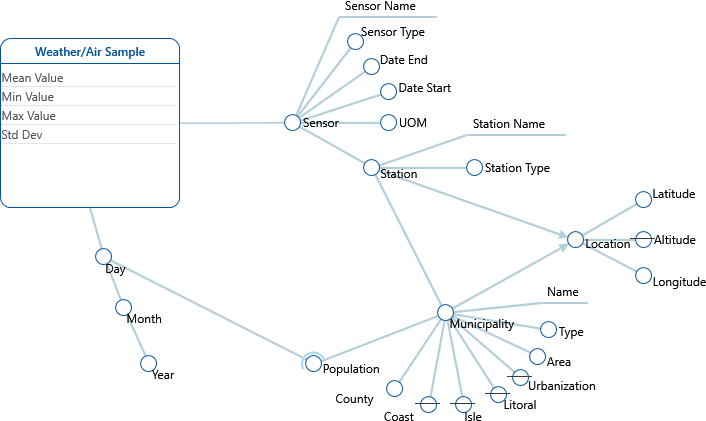
\includegraphics[width=0.6\textwidth]{./images/WeatherAirSampleDFM.png}
		\caption{Weather and Air Quality Sample DFM}
	\end{figure}
	
	\begin{figure}[H]
		\centering
		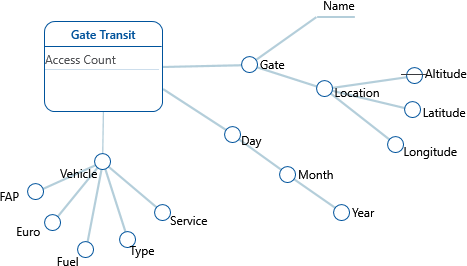
\includegraphics[width=0.6\textwidth]{./images/GateAccessDFM.png}
		\caption{Gate Access DFM}
	\end{figure}
	
	\begin{figure}[H]
		\centering
		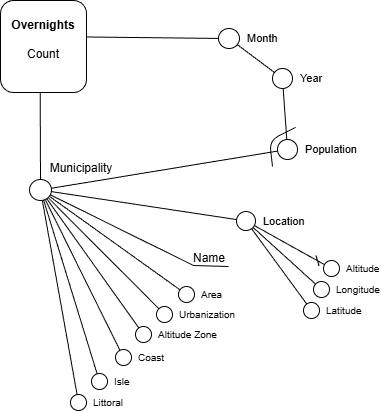
\includegraphics[width=0.5\textwidth]{./images/OvernightsDFM.png}
		\caption{Overnights DFM}
	\end{figure}
	
	\newpage
	\subsection{Snowflake Schema}
	
	The three DFM models were merged into a single \textbf{snowflake schema} instead of three separate star schemas.
	Shared concepts: coordinates (\texttt{location\_dt}), municipality metadata (\texttt{municipality\_dt}), and date (\texttt{date\_dt}) live in dedicated tables that multiple fact tables and dimensions reference.
	This cuts redundancy across \texttt{station\_dt}, \texttt{gate\_dt}, and \texttt{municipality\_dt}, keeps natural hierarchies intact (sensor $\rightarrow$ station $\rightarrow$ municipality $\rightarrow$ location), and makes cross-fact joins possible, for instance linking \texttt{sample\_ft} and \texttt{overnights\_ft} through \texttt{municipality\_dt} without duplicating data.
	
	\begin{figure}[H]
		\centering
		\includegraphics[width=0.8\textwidth]{./images/Schema.png}
	\end{figure}
	
	\newpage
	\subsection{Fact Tables}
	
	\subsubsection{Weather and Air Quality Sample Fact (\textbf{\texttt{sample\_ft}})}
	
	Daily aggregated measurements from a single sensor, either air quality or weather. One row per sensor per day. Time is given by \texttt{date\_dt}; the sensor links through \texttt{sensor\_dt} to its station and municipality.
	\begin{table}[H]
		\centering
		\begin{tabular}{lll}
			\hline
			Column & Type & Description \\
			\hline
			sensor\_id & integer & FK with sensor\_dt \\
			date\_id & integer & FK with date\_dt \\
			mean\_value & double & Daily average measurement \\
			min\_value & double & Daily minimum \\
			max\_value & double & Daily maximum \\
			std\_dev & double & Daily standard deviation \\
			\hline
		\end{tabular}
	\end{table}
	
	\subsubsection{Area C Gate Access Fact (\textbf{\texttt{gate\_access\_ft}})}
	
	Number of transits for a given vehicle profile through a given Area C gate on a given day. One vehicle profile-gate-day combination.
	\begin{table}[H]
		\centering
		\begin{tabular}{lll}
			\hline
			Column & Type & Description \\
			\hline
			gate\_id & integer & FK with gate\_dt \\
			date\_id & integer & FK with date\_dt \\
			vehicle\_id & integer & FK with vehicle\_dt \\
			count & integer & Number of transits \\
			\hline
		\end{tabular}
	\end{table}
	
	\subsubsection{Tourism Overnights Fact (\textbf{\texttt{overnights\_ft}})}
	
	Total overnight stays in a municipality during a given month. One municipality-month combination.
	\begin{table}[H]
		\centering
		\begin{tabular}{lll}
			\hline
			Column & Type & Description \\
			\hline
			municipality\_id & integer & FK with municipality\_dt \\
			month\_id & integer & FK with month\_dt \\
			count & integer & Monthly overnight stays \\
			\hline
		\end{tabular}
	\end{table}
	
	\subsection{Dimension Tables}
	
	\subsubsection{Date Dimension (\textbf{\texttt{date\_dt}})}
	
	Temporal attributes for each daily measurement, breaking a full date into day, month, and year.
	
	\begin{table}[H]
		\centering
		\begin{tabular}{lll}
			\hline
			Column & Type & Description \\
			\hline
			date\_id & integer & Primary key \\
			date & date & Full date \\
			day & smallint & Day of month \\
			month & smallint & Month \\
			year & smallint & Year \\
			\hline
		\end{tabular}
	\end{table}
	
	\subsubsection{Month Dimension (\textbf{\texttt{month\_dt}})}
	
	Month and year, used only by \textbf{\texttt{overnights\_ft}}.
	A separate \textbf{\texttt{month\_dt}} was created instead of reusing \textbf{\texttt{date\_dt}} for two reasons.
	First, tourism data is monthly, there is no day-level detail. Linking \texttt{overnights\_ft} to \texttt{date\_dt} would force every overnight record onto an arbitrary day (say, the first of the month), adding false precision that does not exist in the source.
	Second, joining to \texttt{date\_dt} would blow up each municipality-month row to as many as 31 rows, one per day, wasting storage for zero analytical gain.
	A dedicated \texttt{month\_dt} keeps the fact at its natural grain, respects the snowflake semantics, and avoids pointless overhead.

	\begin{table}[H]
		\centering
		\begin{tabular}{lll}
			\hline
			Column & Type & Description \\
			\hline
			month\_id & integer & Primary key \\
			month & smallint & Month \\
			year & smallint & Year \\
			\hline
		\end{tabular}
	\end{table}
	
	\subsubsection{Location Dimension (\textbf{\texttt{location\_dt}})}
	
	Latitude, longitude, and altitude, shared by municipalities, monitoring stations, and Area C gates. Putting coordinates in one table removes duplication from \texttt{station\_dt}, \texttt{gate\_dt}, and \texttt{municipality\_dt}.
	\begin{table}[H]
		\centering
		\begin{tabular}{lll}
			\hline
			Column & Type & Description \\
			\hline
			location\_id & integer & Primary key \\
			latitude & double precision & Latitude \\
			longitude & double precision & Longitude \\
			altitude & double precision & Altitude in meters (NULL for gates) \\
			\hline
		\end{tabular}
	\end{table}
	
	\subsubsection{Municipality Dimension (\textbf{\texttt{municipality\_dt}})}
	
	Descriptive attributes for every Lombardia municipality: name, urbanization level, area, altimetric zone, coastal and island flags, and a pointer to geographic coordinates in \texttt{location\_dt}.
	\begin{table}[H]
		\centering
		\begin{tabular}{lll}
			\hline
			Column & Type & Description \\
			\hline
			municipality\_id & integer & Primary key \\
			name & varchar(100) & Municipality name \\
			urbanization & varchar(100) & Urbanization level label \\
			area & double & Territory area \\
			littoral & boolean & Coastal municipality flag \\
			isle & boolean & Island municipality flag \\
			coast & boolean & Coastal zone flag \\
			altitude\_zone & varchar(100) & Altimetric zone label \\
			location\_id & integer & FK location\_dt \\
			\hline
		\end{tabular}
	\end{table}
	
	\subsubsection{Station Dimension (\textbf{\texttt{station\_dt}})}
	
	Attributes of air quality and weather monitoring stations. Each station links to its municipality through \texttt{municipality\_dt} and to its coordinates through \texttt{location\_dt}.
	\begin{table}[H]
		\centering
		\begin{tabular}{lll}
			\hline
			Column & Type & Description \\
			\hline
			station\_id & integer & Primary key \\
			name & varchar(100) & Station name \\
			type & varchar(100) & Station type \\
			municipality\_id & integer & FK municipality\_dt \\
			location\_id & integer & FK location\_dt \\
			\hline
		\end{tabular}
	\end{table}
	
	\subsubsection{Sensor Dimension (\textbf{\texttt{sensor\_dt}})}
	
	Individual sensor records, each tied to a station through \texttt{station\_dt}. Includes measurement type, unit, and the operational date range.
	\begin{table}[H]
		\centering
		\begin{tabular}{lll}
			\hline
			Column & Type & Description \\
			\hline
			sensor\_id & integer & Primary key \\
			name & varchar(100) & Sensor name \\
			type & varchar(100) & Measurement type (pollutant or variable) \\
			uom & varchar(20) & Unit of measurement \\
			date\_start & date & First active date \\
			date\_stop & date & Last active date (NULL if still active) \\
			station\_id & integer & FK station\_dt \\
			\hline
		\end{tabular}
	\end{table}
	
	\subsubsection{Gate Dimension (\textbf{\texttt{gate\_dt}})}
	
	Area C access gates, identified by name and linked to their position through \texttt{location\_dt}.
	\begin{table}[H]
		\centering
		\begin{tabular}{lll}
			\hline
			Column & Type & Description \\
			\hline
			gate\_id & integer & Primary key \\
			name & varchar(100) & Gate name \\
			location\_id & integer & FK location\_dt \\
			\hline
		\end{tabular}
	\end{table}
	
	\subsubsection{Vehicle Dimension (\textbf{\texttt{vehicle\_dt}})}
	
	Every distinct vehicle profile seen in the Area C data. Each row is a unique combination of service flag, vehicle type, fuel type, Euro standard, particulate filter, resident status, and Area C class.
	\begin{table}[H]
		\centering
		\begin{tabular}{lll}
			\hline
			Column & Type & Description \\
			\hline
			vehicle\_id & integer & Primary key \\
			service & varchar(100) & Service vehicle flag \\
			type & varchar(100) & Vehicle type \\
			fuel & varchar(100) & Fuel type \\
			euro & varchar(100) & Euro emission standard \\
			fap & varchar(100) & Particulate filter flag \\
			allowed & varchar(100) & Exempt from Area C flag \\
			resident & varchar(100) & Resident flag \\
			category & varchar(100) & Vehicle category \\
			class & varchar(100) & Area C vehicle class \\
			\hline
		\end{tabular}
	\end{table}
	
	\subsubsection{Population Dimension (\textbf{\texttt{population\_dt}})}
	
	Annual resident population per municipality. Links a municipality to a reference year via \texttt{date\_dt}.
	\begin{table}[H]
		\centering
		\begin{tabular}{lll}
			\hline
			Column & Type & Description \\
			\hline
			population\_id & integer & Primary key \\
			municipality\_id & integer & FK municipality\_dt \\
			date\_id & integer & FK date\_dt \\
			population & integer & Total resident population \\
			\hline
		\end{tabular}
	\end{table}
	

	\newpage
	\section{ETL Flow}

	The ETL pipeline is written in Python, relying on standard libraries for database access and data manipulation.
	It is fully idempotent: every run drops and recreates the entire schema from scratch, so the result is always clean and reproducible.
	All datasets were downloaded manually and saved locally because not every source offers a direct download URL. Multi-year files were pre-filtered to 2023 to keep memory usage and runtime reasonable.

	Three abstract base classes give the pipeline its structure.

	\begin{lstlisting}[language=Python]
@dataclass
class Pipeline(ABC):

	def run(self):
		self.extract()
		self.transform()
		self.load()

	@abstractmethod 
	def extract(self): pass

	@abstractmethod
	def transform(self): pass

	@abstractmethod
	def load(self): pass

	@abstractmethod
	def get_df(self) -> pd.DataFrame: pass
	\end{lstlisting}

	\texttt{Pipeline} defines the extract-transform-load lifecycle. Concrete subclasses fill in the three steps for one target table each.

	\begin{lstlisting}[language=Python]
@dataclass
class Table(ABC):

	@abstractmethod
	def get_id(self, *args, **kwargs): pass
	\end{lstlisting}

	Once a pipeline finishes, its output DataFrame is wrapped in a \texttt{Table} subclass. The \texttt{get\_id} method on each subclass contains the lookup logic for that table; downstream pipelines call it to resolve foreign keys.

	\begin{lstlisting}[language=Python]
@dataclass
class Source(ABC):

	@abstractmethod
	def extract(self) -> pd.DataFrame: pass
	\end{lstlisting}

	\texttt{Source} wraps a raw data file. Subclasses store format-specific details (delimiter, encoding) and cache the loaded DataFrame so that two pipelines reading the same file do not parse it twice.

	\subsection{Extraction Phase}

	Raw CSVs are loaded through typed \texttt{Source} subclasses. The resulting DataFrame goes straight to the transformation step.

	\subsection{Transformation Phase}

	Each pipeline takes the \texttt{Source} objects it needs and the \texttt{Table} objects of already-loaded dimensions. It outputs a cleaned DataFrame ready for loading. The transformation steps are:

	\begin{itemize}
		\item \textbf{Filtering and validation:} dropping invalid or out-of-scope records measurements with the missing-value sentinel, inactive sensors, entries outside 2023.
		\item \textbf{Schema harmonization:} renaming and selecting columns so that heterogeneous sources share one schema before any join or concatenation.
		\item \textbf{Code decoding:} replacing numeric or abbreviated codes with readable labels through lookup tables (e.g.\ urbanization levels, altimetric zones, Area C vehicle fields). Not every table needed this.
		\item \textbf{Temporal aggregation:} rolling data up to the target granularity. Sensor samples, for instance, are aggregated to daily level with mean, min, max, and standard deviation. Not every table needed it.
		\item \textbf{Foreign-key resolution:} matching each record to its dimension surrogate key. Where a plain join is not enough, the \texttt{get\_id} method of the relevant \texttt{Table} handles the lookup, keeping resolution logic out of the pipeline code.
		\item \textbf{Referential integrity enforcement:} any row whose foreign key cannot be resolved is dropped, so no orphan records reach the database.
	\end{itemize}

	Because the snowflake schema creates dependencies between dimension tables, pipelines run in dependency order: each table is fully loaded before any downstream pipeline tries to resolve keys against it.

	\subsection{Load Phase}

	Each pipeline's \texttt{load} method writes its DataFrame to the target table. Dimensions are loaded first, then fact tables, respecting FK dependencies.

	\newpage
	\section{Analysis}
	
	Each analysis targets one of the business questions from Section 2, using a mix of Advanced SQL, Association Rule Mining, and Machine Learning Algorithms.

	\subsection{How can air quality data across municipalities be analyzed to support environmental and public health decision-making?}
	
	\subsubsection{Which urbanization levels show the highest pollutant concentrations?}
	
	Four pollutants are considered: \textbf{NO$_2$}, \textbf{PM$_{10}$}, \textbf{PM$_{2.5}$}, and \textbf{O$_3$}. Each is compared against the WHO 2021 daily guideline values (\href{https://www.who.int/publications/i/item/9789240034228}{source}):
	
	\begin{table}[H]
		\centering
		\begin{tabular}{ll}
			\hline
			Pollutant & Concentration ($\mu$g/m$^3$) \\
			\hline
			NO$_2$    & 25 \\
			PM$_{10}$   & 45 \\
			PM$_{2.5}$  & 15 \\
			O$_3$     & 100 \\
			\hline
		\end{tabular}
		\caption{Air Quality Thresholds}
	\end{table}
		
	ISTAT classifies municipalities into three urbanization levels: \textbf{Dense}, \textbf{Intermediate}, and \textbf{Rural}. 
	Statistics were computed per pollutant and urbanization level and compared to the Lombardia-wide aggregate.
	
	\begin{figure}[H]
		\centering
		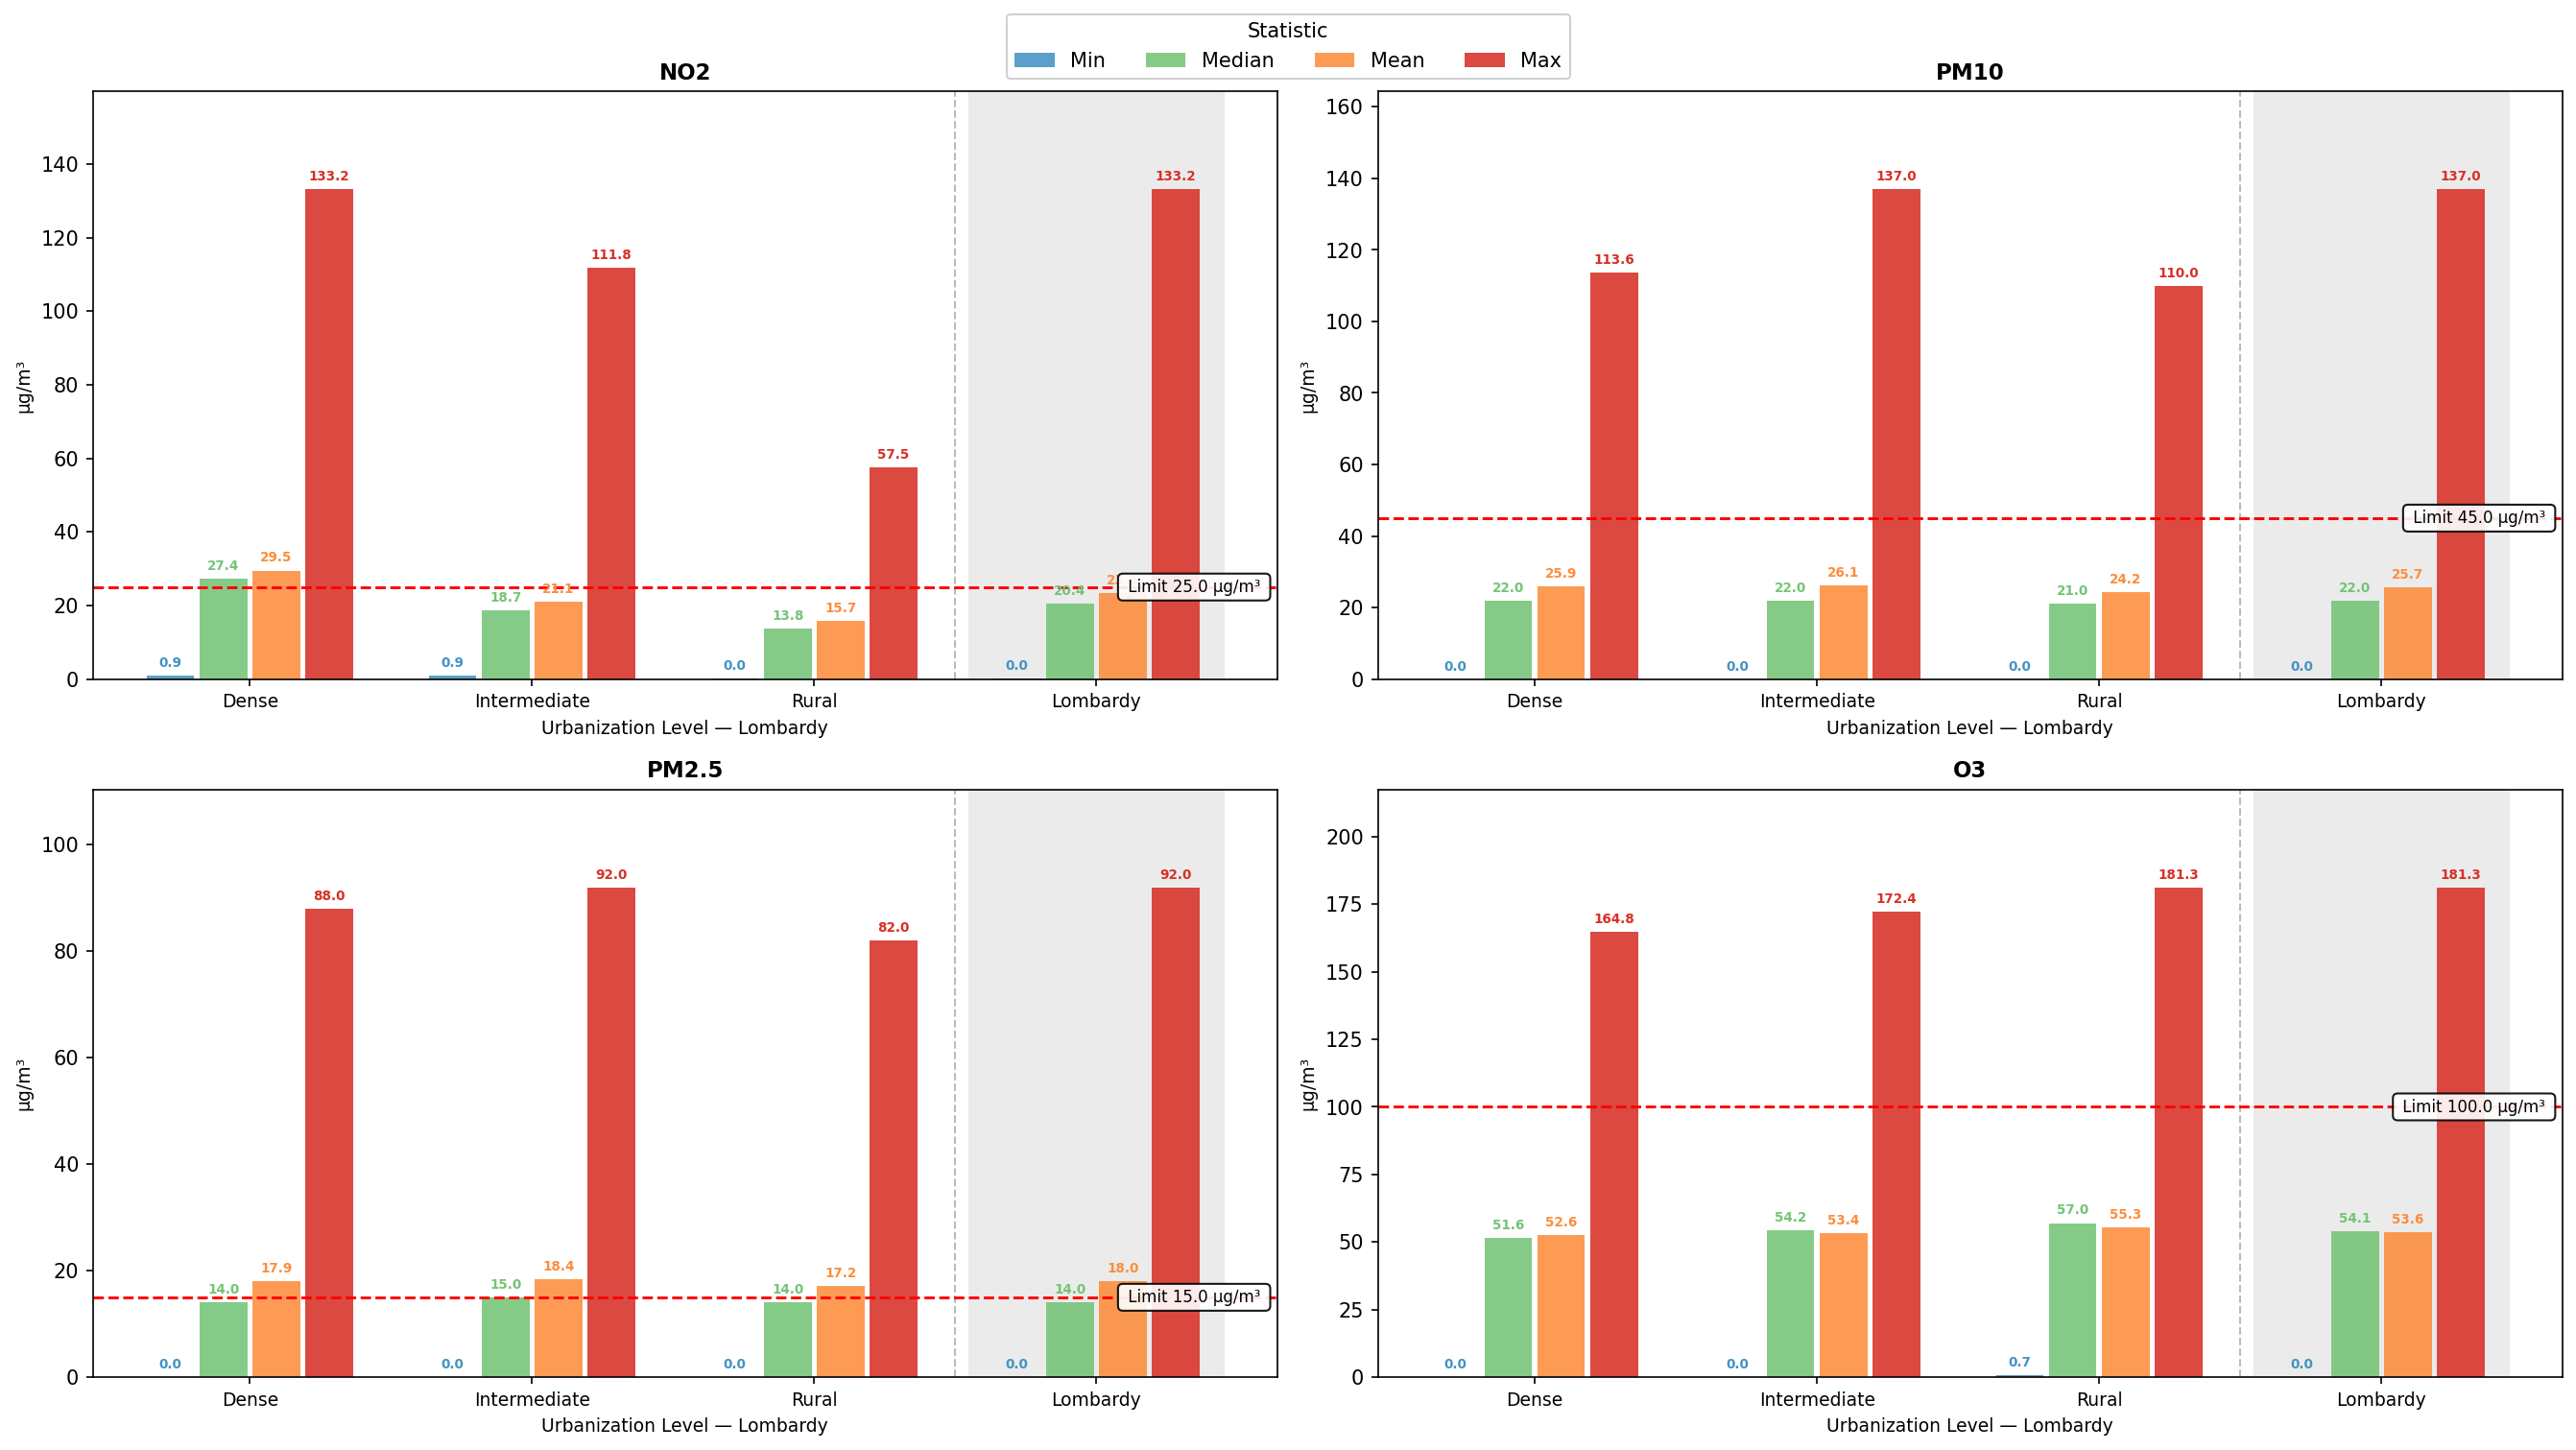
\includegraphics[width=\textwidth]{./images/1_air_quality/hierarchical_stats_combined.png}
	\end{figure}

	Particulate matter (\textbf{PM${10}$} and \textbf{PM${2.5}$}) is a \textbf{regional rather than urban problem}, lacking a clear urbanization gradient and even peaking in \textbf{Intermediate} areas. 
	\textbf{PM$_{2.5}$} is uniquely critical as it uniformly exceeds annual limits everywhere, demanding region-wide structural measures instead of local fixes.
	Pollutant patterns vary across urbanization levels. Dense areas are characterized by higher \textbf{NO$_2$} concentrations, rural areas by elevated \textbf{O$_3$} levels linked to reduced NO titration, 
	while intermediate zones show the highest \textbf{PM$_{10}$} and \textbf{PM$_{2.5}$} concentrations.

	\subsubsection{Are there municipalities that repeatedly experience multi-day episodes of pollution above health-based thresholds?}
	
	To find municipalities with recurring sustained exceedances, \textbf{critical pollution windows} were defined: consecutive days on which a municipality's daily average stays above the threshold for a given pollutant.
	The charts show the top 10 longest consecutive exceedance episodes per pollutant; darker red means longer duration.
	\begin{figure}[H]
		\centering
		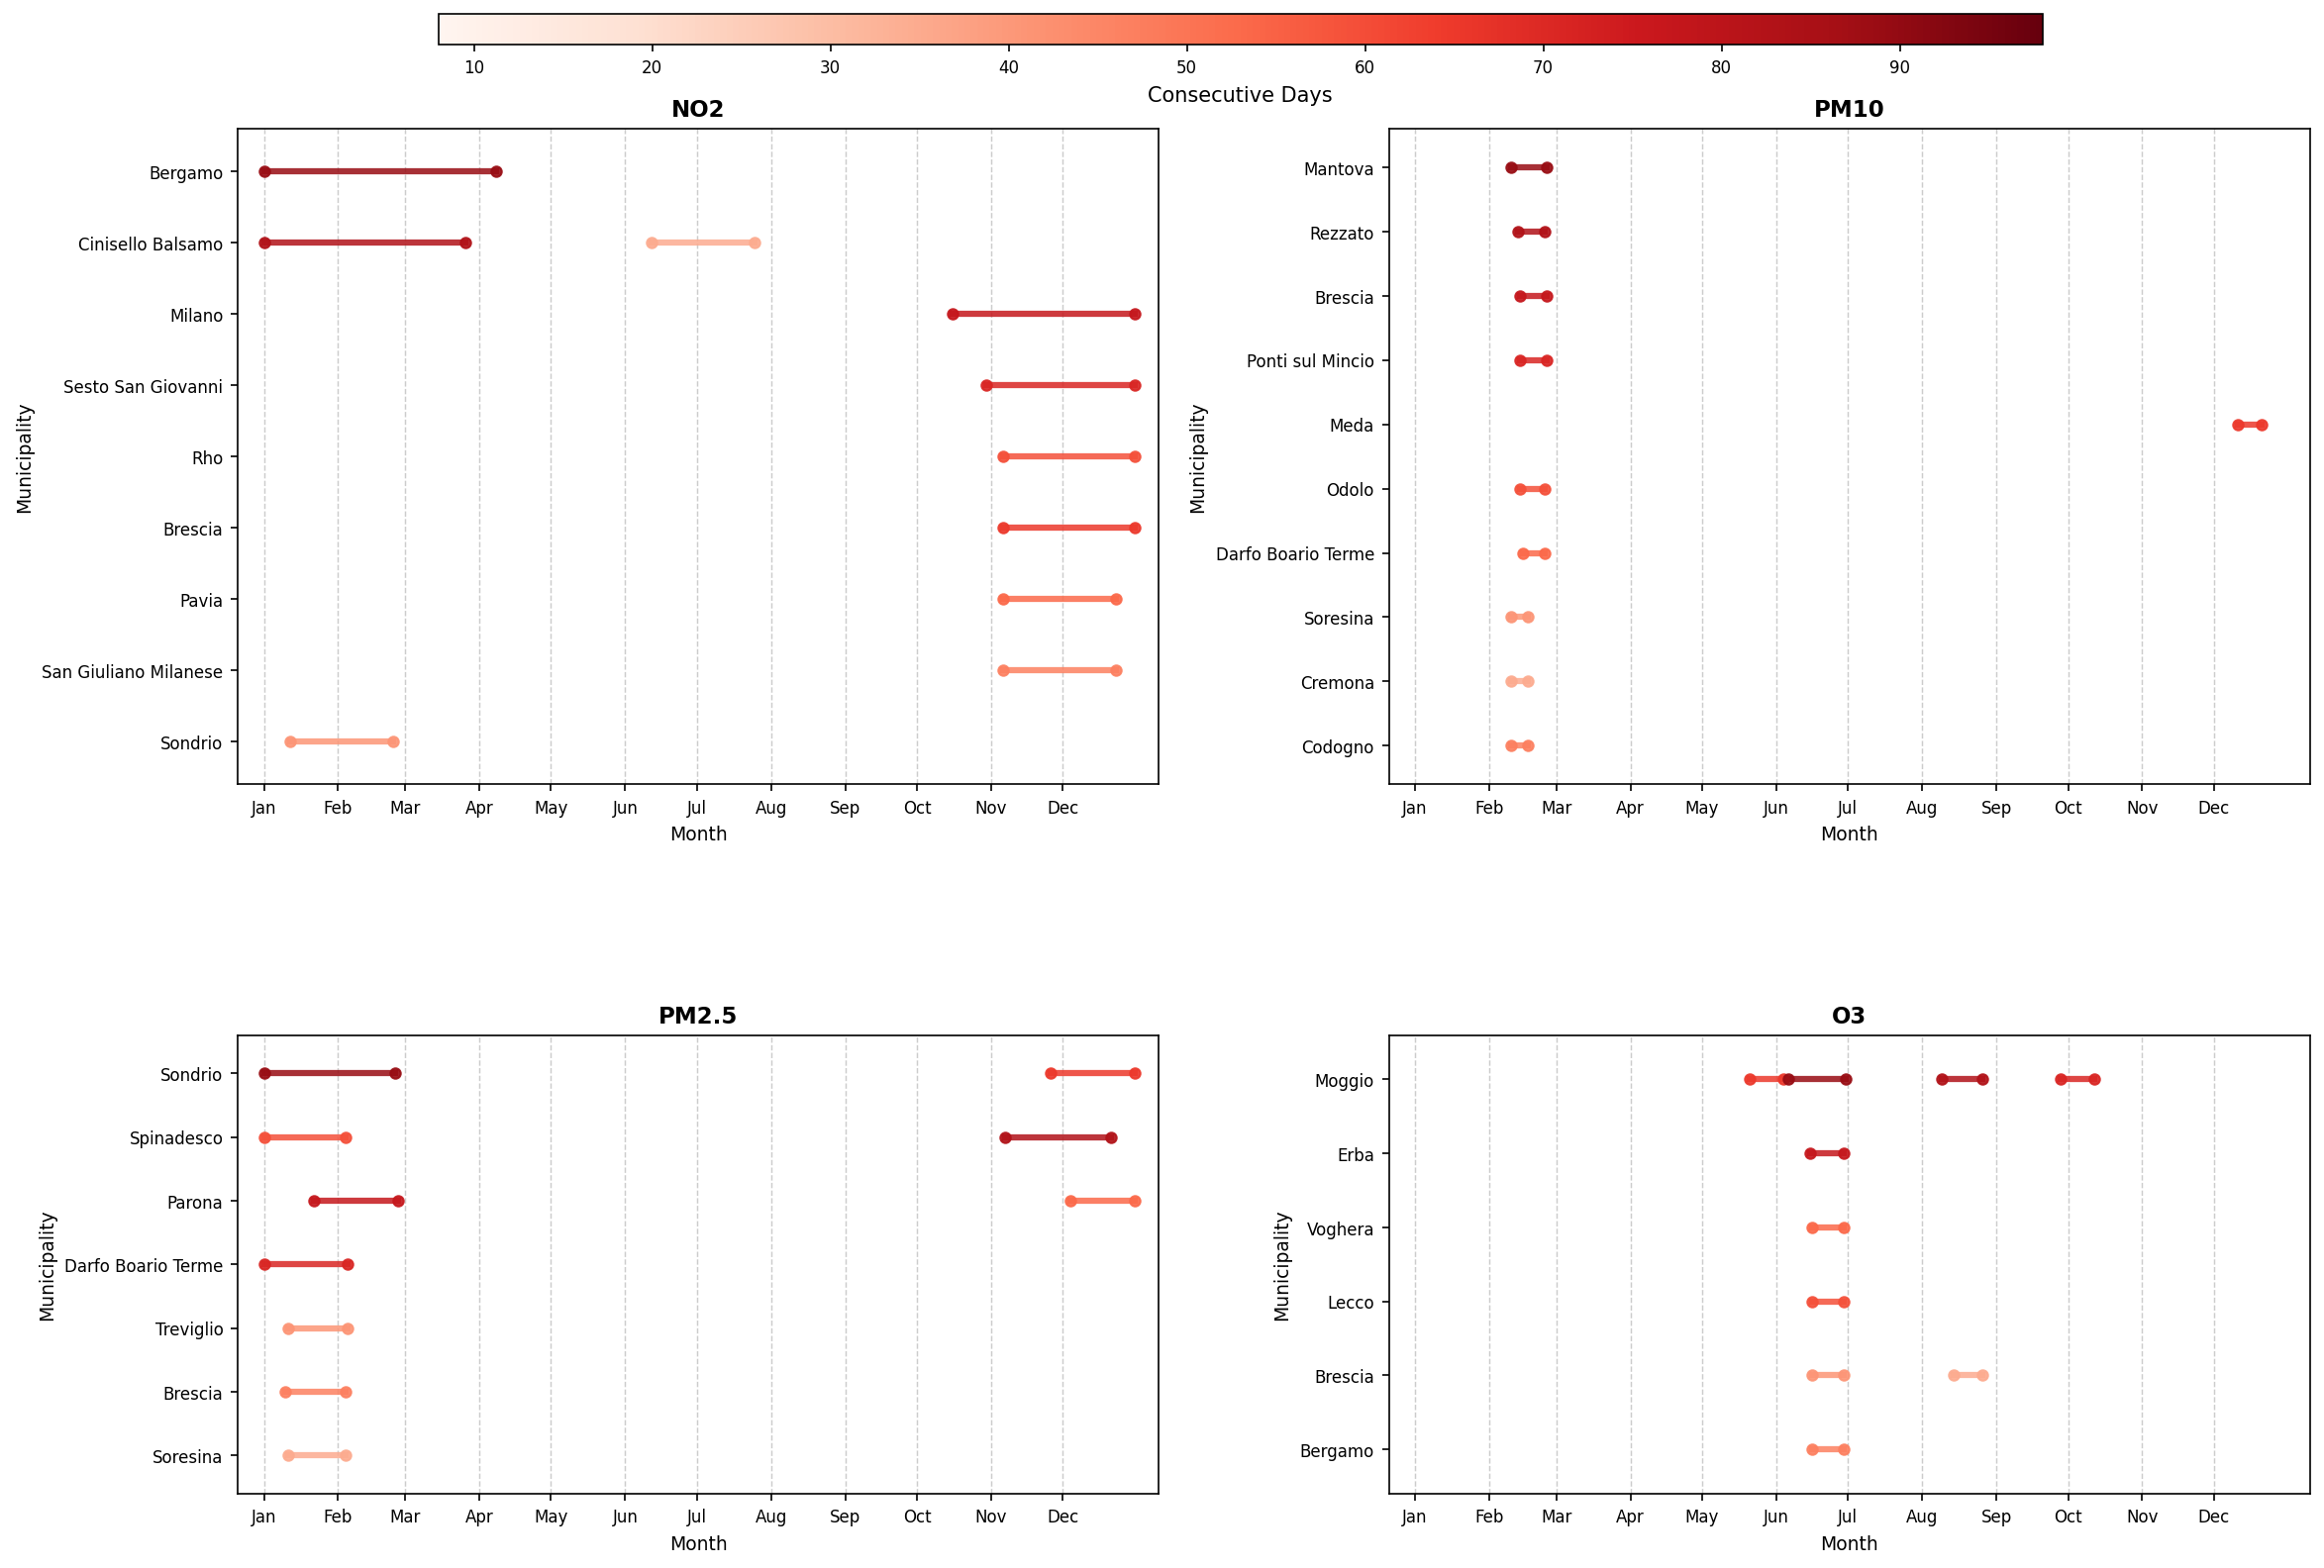
\includegraphics[width=\textwidth]{./images/1_air_quality/critical_episodes_combined.png}
	\end{figure}
	
	 Exceedances cluster in predictable calendar windows.

	Two cases break the pattern. \textbf{Cinisello Balsamo} registers an NO$_2$ episode in mid-summer, when traffic is typically low. That is unusual and suggests a local non-traffic source. \textbf{Moggio} shows O$_3$ exceedances from May all the way to October far longer than anywhere else. 

	Episode duration matters as much as frequency. A week-long exceedance is a different health risk from a one-day spike, and any risk assessment should weight it accordingly.
			
	\subsubsection{Can municipalities be grouped based on their pollution profile?}
	
	\textbf{K-Means Clustering} was run on daily pollution profiles to group municipalities. The feature matrix contains the daily average concentration of NO$_2$, PM$_{10}$, PM$_{2.5}$, and O$_3$, effectively a 365-day time series per pollutant for each municipality. Municipalities with less than 50\% daily coverage across the full matrix were dropped. Missing values in the remaining rows were filled with the \textbf{column median}, that is, the region-wide daily median for that pollutant on that day. A stricter filter demanding all four pollutants would have left too few municipalities to cluster usefully. Features were scaled with a \textbf{Robust Scaler} to dampen outlier effects.

	$k = 3$ was chosen after inspecting the Elbow Chart, Silhouette Score, and Davies-Bouldin Index.

	For each cluster, weekly averages were plotted against guideline thresholds. A \textbf{Cluster Pollution Index}, the mean per-pollutant concentration normalized by its threshold, was computed to rank clusters from dirtiest to cleanest.

	\textbf{Cluster characterization}\\

	\begin{figure}[H]
		\centering
		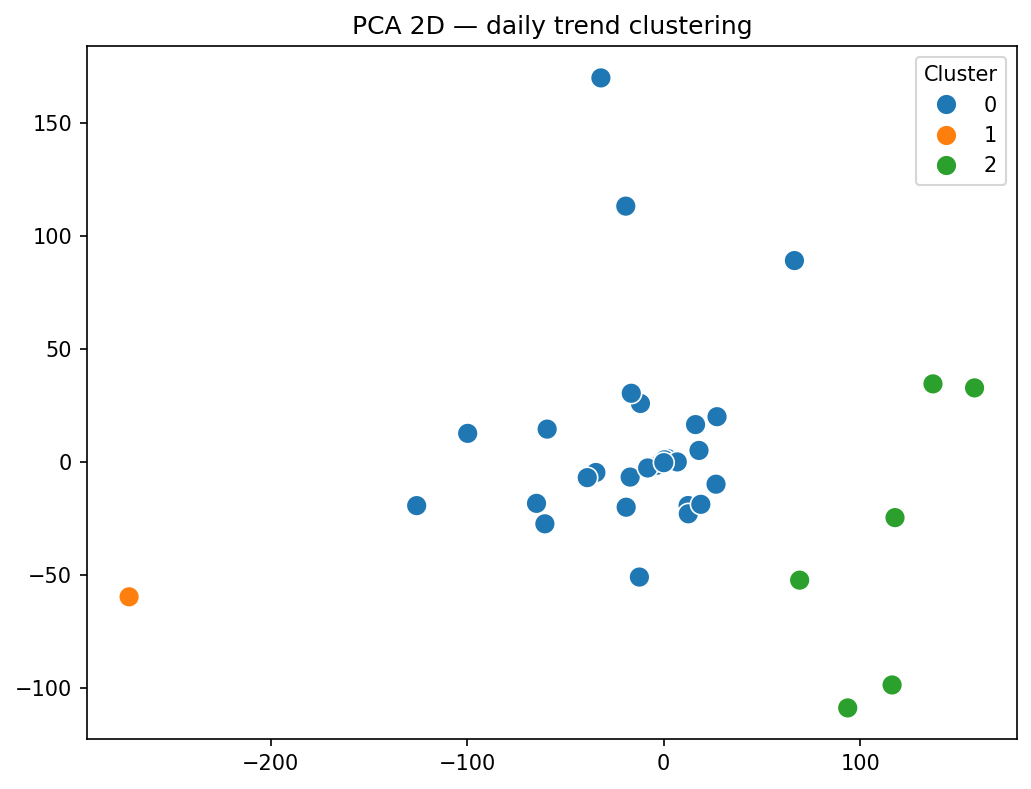
\includegraphics[width=0.8\textwidth]{./images/1_air_quality/cluster_pca.png}
		\caption{2D PCA projection}
	\end{figure}
	
	\begin{figure}[H]
		\centering
		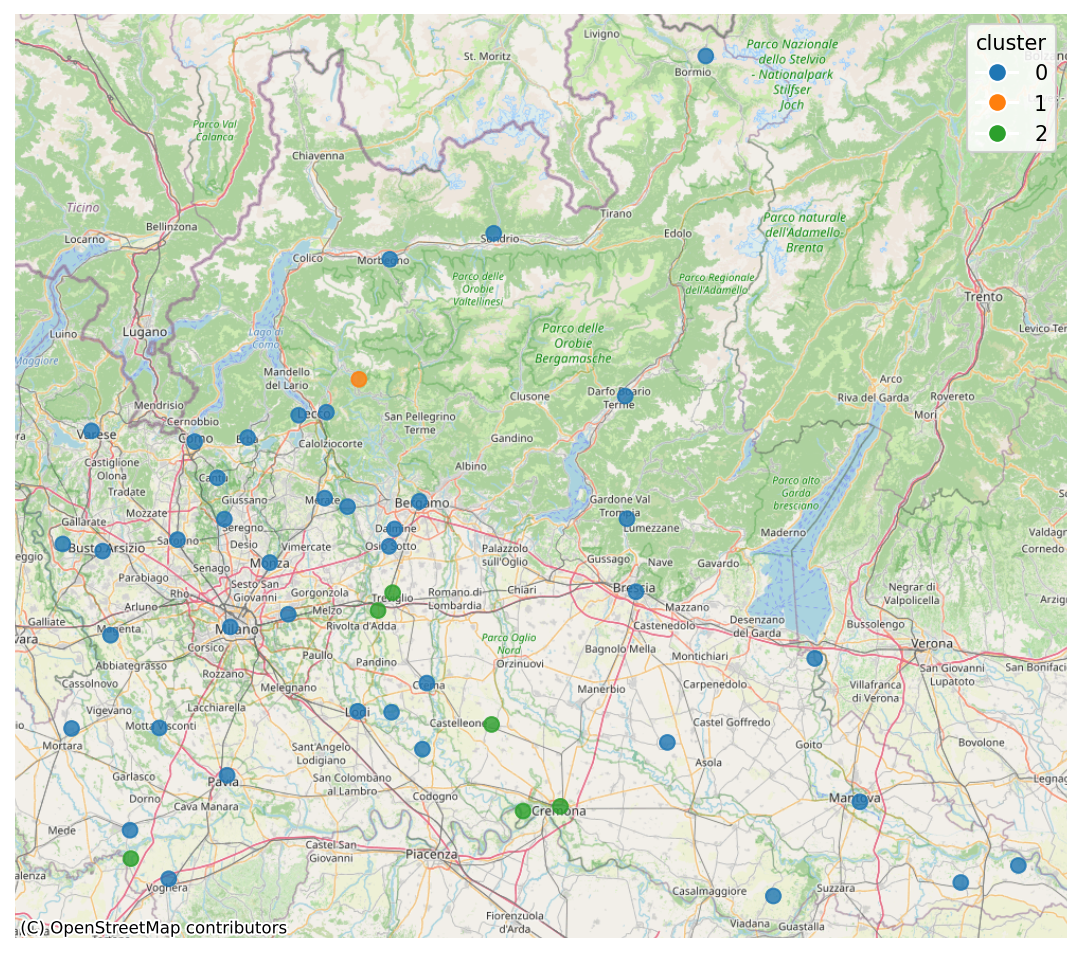
\includegraphics[width=0.8\textwidth]{./images/1_air_quality/cluster_geo_map.png}
		\caption{Cluster location map}
	\end{figure}

	\textbf{Cluster 0} contains most of the monitored municipalities. \textbf{Cluster 2} picks up a smaller, more polluted subset. \textbf{Cluster 1} consists of a \textbf{single municipality}: its profile is so different from everything else that it ends up alone. It is best read as an outlier, not a representative group.
	
	\newpage
	\textbf{Weekly Seasonal trends} \\
	\begin{figure}[H]
		\centering
		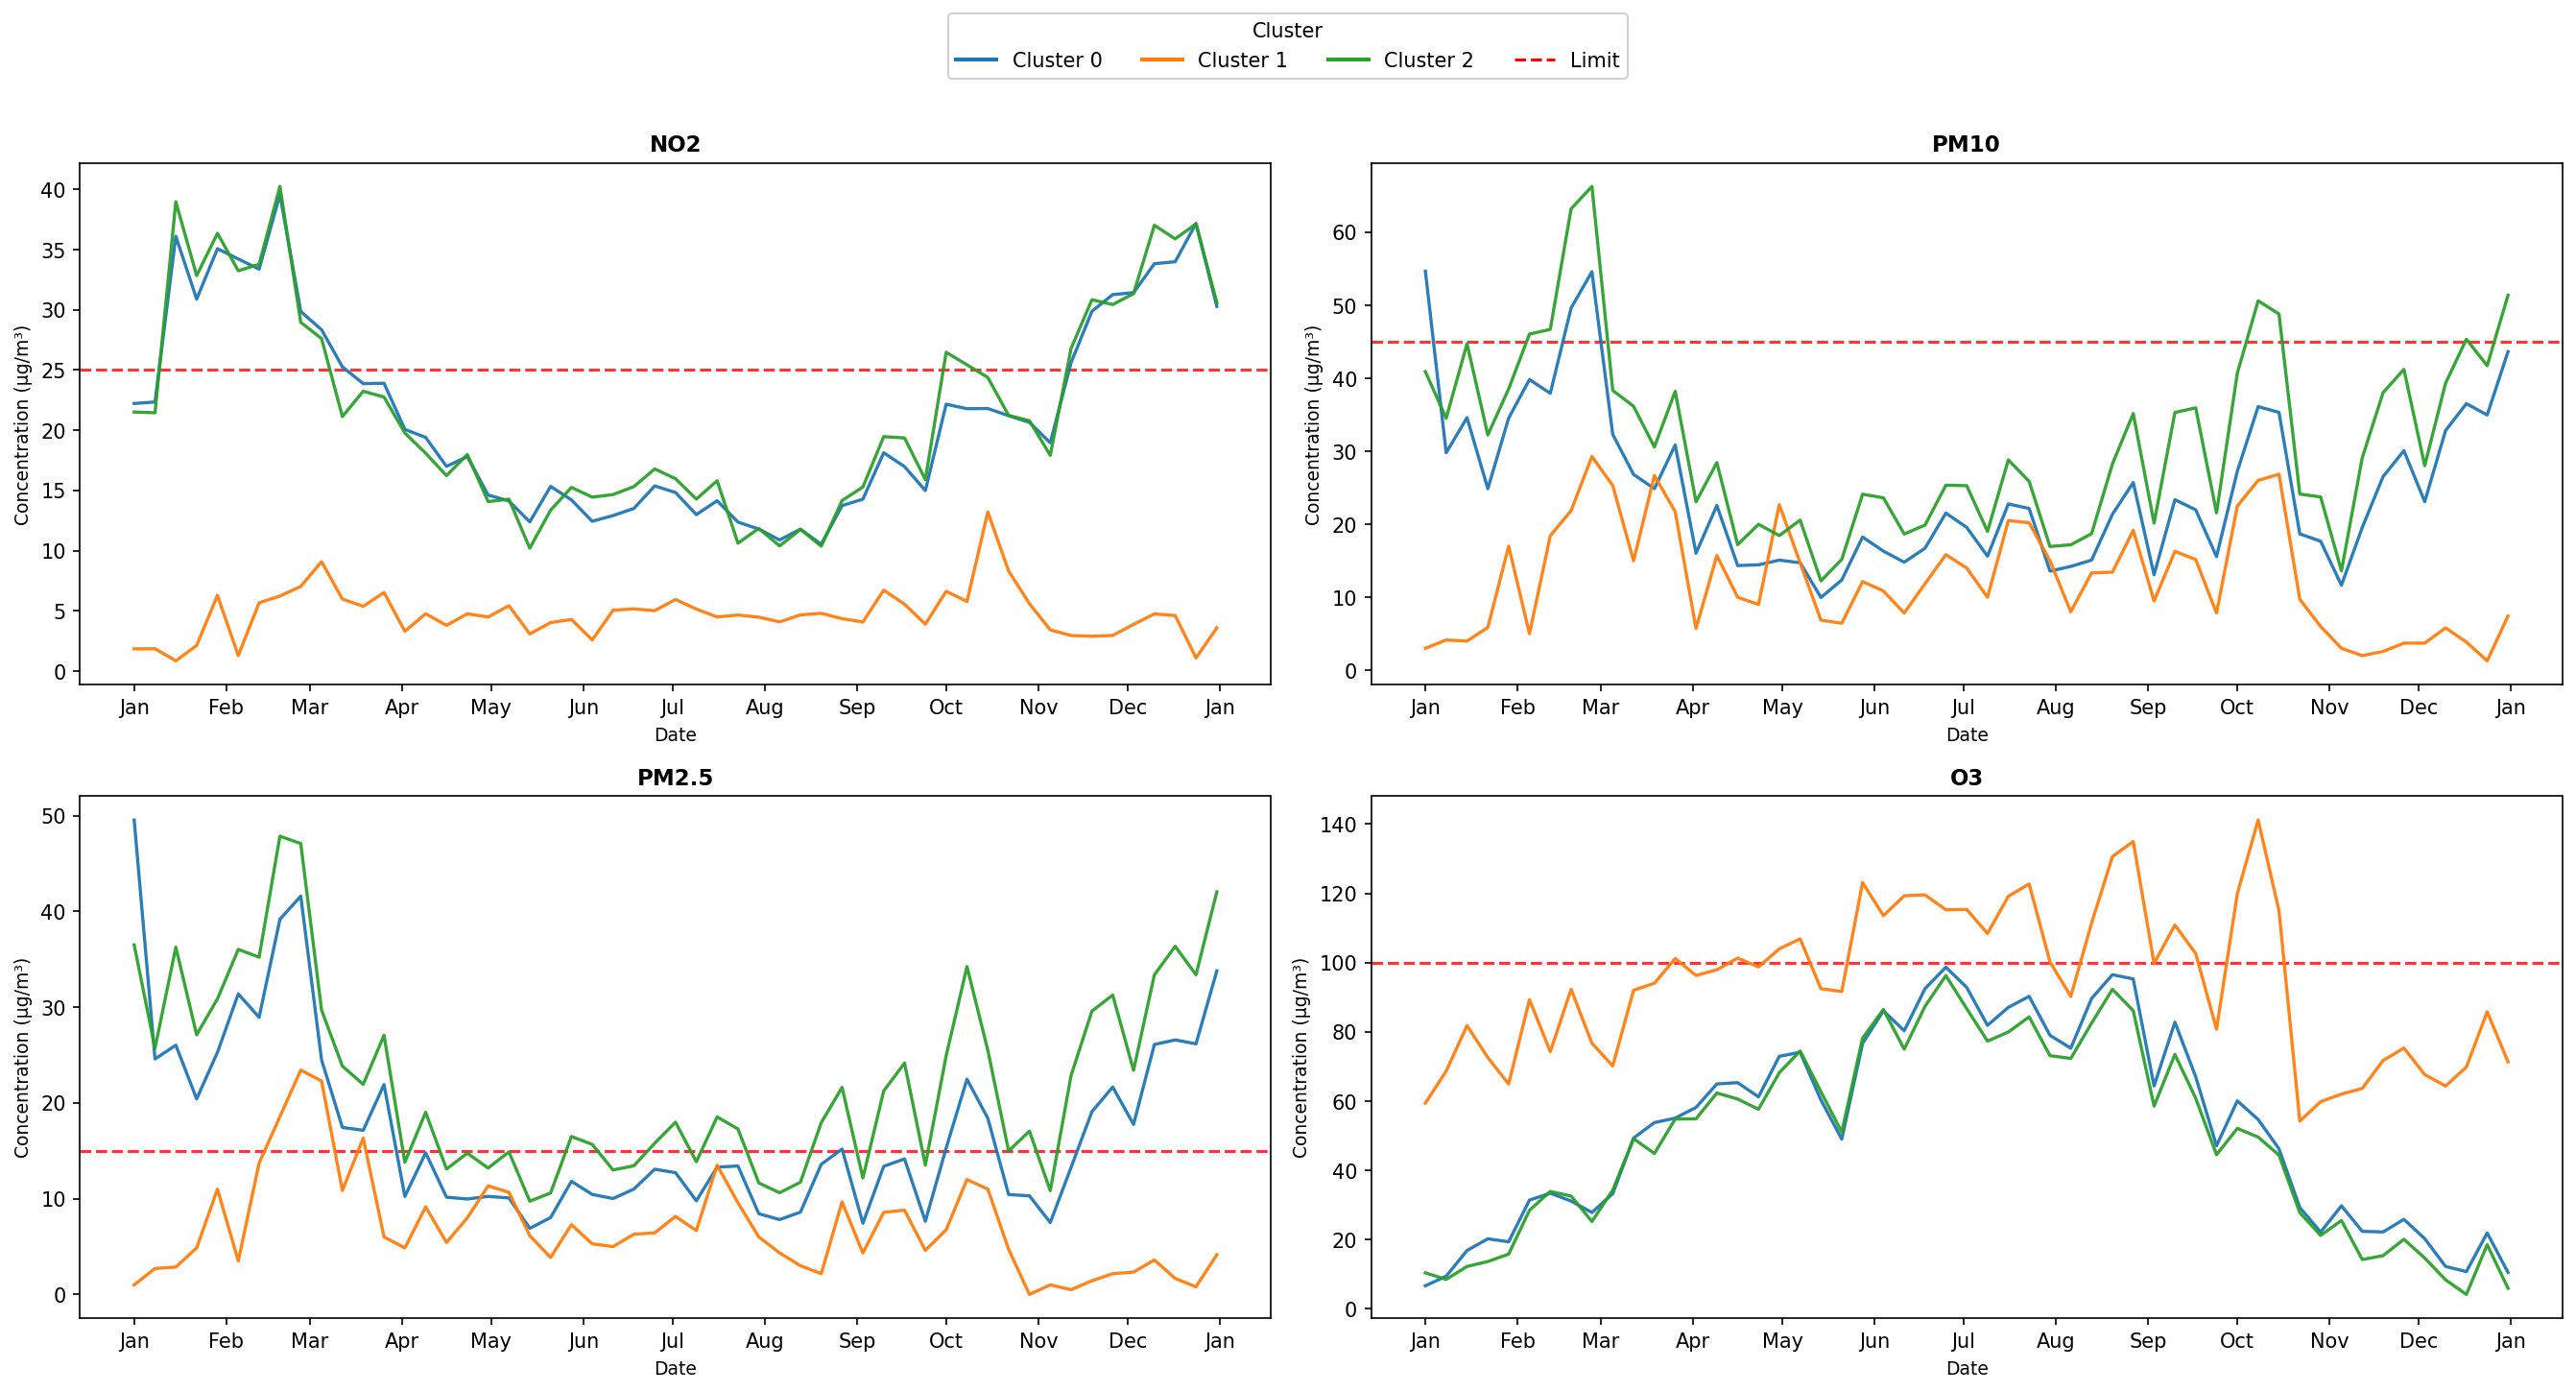
\includegraphics[width=\textwidth]{./images/1_air_quality/cluster_trend_combined.png}
		\caption{Weekly pollutants trend.}
	\end{figure}
	
	The seasonal shape is similar everywhere, primary pollutants (NO$_2$, PM$_{10}$, PM$_{2.5}$) peak in winter and drop through spring and summer; O$_3$ does the opposite, peaking in summer.

	\textbf{Cluster 2} is the more polluted group. Its primary-pollutant concentrations are the highest year-round, and in winter both PM$_{2.5}$ and NO$_2$ regularly breach guideline levels.
	\textbf{Cluster 0} sits near the regional average. 
	\textbf{Cluster 1}, the lone municipality, has readings extreme enough to form its own cluster, confirming it is a statistical outlier.
	
	\textbf{Cluster Pollution Index} \\
	\begin{table}[H]
		\centering
		\begin{tabular}{lr}
			\hline
			Cluster & Pollution Index \\
			\hline
			2 & 0.887 \\
			0 & 0.779 \\
			1 & 0.471 \\
			\hline
		\end{tabular}
		\caption*{Cluster Pollution Index.}
	\end{table}

	 \textbf{Cluster 2} has the highest index (0.887). \textbf{Cluster 0} comes next at 0.779. \textbf{Cluster 1} is well below at 0.471.
	
	\newpage
	\subsubsection{Which municipalities are most polluted with particulate matter?}

	The top 5 most particulate-polluted municipalities were extracted month by month for PM$_{2.5}$ and PM$_{10}$. Appearances were then broken down by urbanization level and compared to the baseline distribution of monitored municipalities (23\% Dense, 56\% Intermediate, 21\% Rural).

	\textbf{Top 5 municipalities per month PM$_{2.5}$}

	\begin{table}[H]
		\centering
		\resizebox{\textwidth}{!}{%
		\begin{tabular}{llllll}
			\hline
			Month & 1\textsuperscript{st} & 2\textsuperscript{nd} & 3\textsuperscript{rd} & 4\textsuperscript{th} & 5\textsuperscript{th} \\
			\hline
			January & Spinadesco & Soresina& Darfo Boario Terme & Treviglio & Cremona\\
			February& Ponti sul Mincio & Mantova & Soresina & Spinadesco& Brescia\\
			March & Soresina & Casirate d'Adda & Spinadesco & Bergamo & Treviglio\\
			April & Spinadesco & Casirate d'Adda & Dalmine& Soresina& Treviglio\\
			May & Bergamo& Spinadesco& Casirate d'Adda& Treviglio & Pavia\\
			June& Dalmine& Treviglio & Casirate d'Adda& Spinadesco& Saronno\\
			July& Casirate d'Adda& Cornale e Bastida & Soresina & Cremona & Spinadesco \\
			August& Spinadesco & Soresina& Casirate d'Adda& Cremona & Cornale e Bastida\\
			September & Casirate d'Adda& Soresina& Spinadesco & Cremona & Cornale e Bastida\\
			October & Soresina & Cornale e Bastida & Spinadesco & Casirate d'Adda & Treviglio\\
			November& Spinadesco & Soresina& Cremona& Cornale e Bastida & Casirate d'Adda\\
			December& Soresina & Spinadesco& Cremona& Monza & Casirate d'Adda\\
			\hline
		\end{tabular}}
		\caption*{PM$_{2.5}$ top-5 appearances.}
	\end{table}

	\begin{table}[H]
		\centering
		\begin{tabular}{lrr}
			\hline
			Urbanization & Appearances & Share (\%) \\
			\hline
			Dense& 12& 20.0 \\
			Intermediate & 31& 51.7 \\
			Rural& 17& 28.3 \\
			\hline
		\end{tabular}
		\caption*{PM$_{2.5}$ top-5 appearances by urbanization level.}
	\end{table}

	\textbf{Top 5 municipalities per month PM$_{10}$}

	\begin{table}[H]
		\centering
		\resizebox{\textwidth}{!}{%
		\begin{tabular}{llllll}
			\hline
			Month & 1\textsuperscript{st} & 2\textsuperscript{nd} & 3\textsuperscript{rd} & 4\textsuperscript{th} & 5\textsuperscript{th} \\
			\hline
			January & Darfo Boario Terme & Rezzato & Soresina& Codogno & Meda \\
			February& Rezzato& Mantova & Ponti sul Mincio & Brescia & Soresina \\
			March & Rezzato& Soresina& Codogno & Brescia & Casirate d'Adda\\
			April & Spinadesco & Soresina& Casirate d'Adda & Dalmine & Darfo Boario Terme \\
			May & Spinadesco & Soresina& Codogno & Casirate d'Adda & Brescia\\
			June& Borgocarbonara & Spinadesco& Codogno & Rezzato & Soresina \\
			July& Borgocarbonara & Spinadesco& Soresina& Casirate d'Adda & Codogno\\
			August& Soresina & Codogno & Spinadesco& Crema & Borgocarbonara \\
			September & Soresina & Spinadesco& Casirate d'Adda & Cremona & Crema\\
			October & Soresina & Codogno & Rezzato & Crema & Spinadesco \\
			November& Soresina & Rezzato & Spinadesco& Codogno & Cremona\\
			December& Rezzato& Meda& Soresina& Mantova & Cremona\\
			\hline
		\end{tabular}}
		\caption*{PM$_{10}$ top-5 appearances.}
	\end{table}

	\begin{table}[H]
		\centering
		\begin{tabular}{lrr}
			\hline
			Urbanization & Appearances & Share (\%) \\
			\hline
			Dense& 8 & 13.3 \\
			Intermediate & 41& 68.3 \\
			Rural& 11& 18.3 \\
			\hline
		\end{tabular}
		\caption*{PM$_{10}$ top-5 appearances by urbanization level.}
	\end{table}

	Dense municipalities are \textbf{under-represented} relative to their share of the monitoring network. Intermediate and Rural areas are \textbf{over-represented} for both pollutants.

	The gap is widest for PM$_{10}$, Intermediate municipalities make up 68.3\% of appearances versus a 56\% baseline, while Dense areas drop to 13.3\% against 23\%. 
	One plausible reading is that urban traffic restrictions and centralized heating regulations are doing their job in large cities, but peripheral industrial and agricultural zones remain outside current policy reach.

	For PM$_{2.5}$, Rural municipalities appear in 28.3\% of slots versus a 21\% baseline. That over-representation fits indrustrial and agricultural emissions, sources that urban air quality frameworks barely touch. 

	\newpage
	
	\subsection{How do weather variables relate to pollutant concentrations across municipalities?}

	\subsubsection{Which weather variables are most strongly correlated with pollutant concentrations?}

	\textbf{Pearson correlation coefficients} were computed between daily weather variables (temperature, humidity, solar radiation, wind speed, precipitation) and daily pollutant concentrations at municipality level.
	
	\begin{figure}[H]
		\centering
		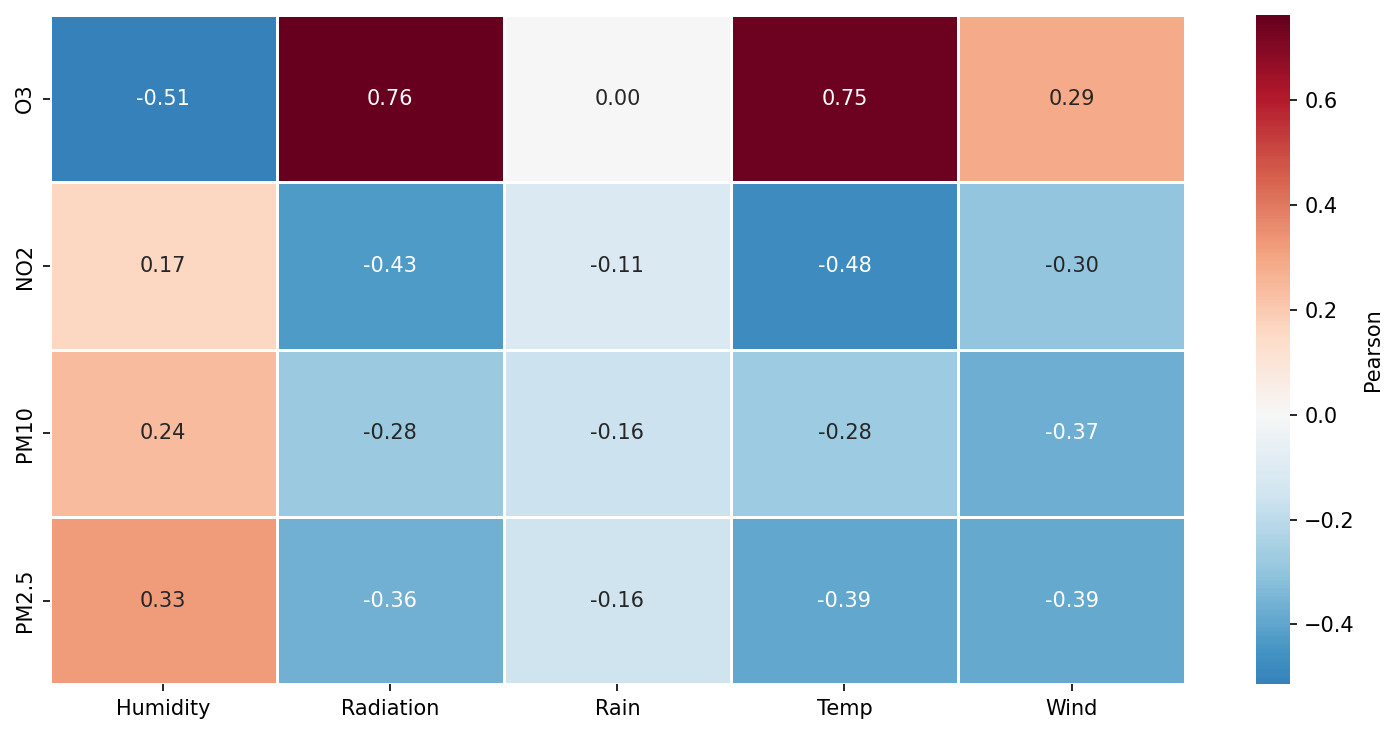
\includegraphics[width=0.7\textwidth]{./images/2_weather_pollution/correlation_heatmap.png}
	\end{figure}
	
	 \textbf{O$_3$} correlates strongly with radiation and temperature (0.76 and 0.75), no surprise given its photochemical origin. The primary pollutants (NO$_2$, PM$_{10}$, PM$_{2.5}$) go the other way, showing negative correlations with the same variables: they accumulate under cold, stagnant, low-radiation conditions.

	 \textbf{Humidity} is the only variable that flips sign across pollutant groups: positive for particulates (up to 0.33 for PM$_{2.5}$), negative for O$_3$ ($-0.51$). At daily resolution, humidity apparently helps PM accumulate rather than washing it out. \textbf{Rain}, on the other hand, is nearly uncorrelated with everything (0.00 to $-0.16$). Precipitation by itself is a poor predictor of air quality.

	\newpage
	\subsubsection{Which combinations of weather conditions frequently co-occur with pollution levels?}

	\textbf{Association Rule Mining} was used to find which weather combinations tend to appear together with specific pollution levels, picking up non-linear and multi-variable patterns that Pearson coefficients miss.\\
	Both weather and pollutant variables were discretized into three ordinal bins (LOW, MID, HIGH) using \textbf{per-municipality tertiles}, so thresholds reflect local conditions.\\
	Apriori was run on the resulting binary matrix with minimum support 0.5\% and minimum confidence 20\%; only rules with lift $\geq$ 1.00 and a weather-only antecedent mapping to a pollutant-only consequent were kept.

	\begin{table}[H]
		\centering
		\resizebox{\textwidth}{!}{%
		\begin{tabular}{llrrr}
			\hline
			Antecedent & Consequent & Support & Confidence & Lift \\
			\hline
			\texttt{RADIATION\_MID + RAIN\_LOW + TEMP\_MID + WIND\_LOW}& \texttt{O3\_MID + PM10\_HIGH} & 0.64\% & 37.1\% & 7.37 \\
			\texttt{RAIN\_LOW + TEMP\_HIGH + WIND\_LOW}& \texttt{O3\_HIGH + PM10\_HIGH}& 0.75\% & 23.1\% & 6.90 \\
			\texttt{HUMIDITY\_MID + RADIATION\_MID + RAIN\_LOW + WIND\_LOW}& \texttt{NO2\_HIGH + O3\_MID + PM10\_HIGH} & 0.57\% & 21.7\% & 6.81 \\
			\texttt{HUMIDITY\_MID + RAIN\_LOW + TEMP\_MID + WIND\_LOW} & \texttt{O3\_MID + PM10\_HIGH} & 0.62\% & 33.8\% & 6.72 \\
			\texttt{HUMIDITY\_MID + RADIATION\_MID + WIND\_LOW}& \texttt{NO2\_HIGH + O3\_MID + PM10\_HIGH} & 0.59\% & 20.5\% & 6.45 \\
			\texttt{HUMIDITY\_MID + RADIATION\_MID + RAIN\_LOW + TEMP\_MID}& \texttt{NO2\_HIGH + O3\_MID + PM10\_HIGH} & 0.50\% & 20.5\% & 6.43 \\
			\texttt{HUMIDITY\_HIGH + RADIATION\_LOW + RAIN\_HIGH + TEMP\_MID}& \texttt{O3\_LOW + PM10\_LOW}& 0.65\% & 23.6\% & 6.30 \\
			\texttt{HUMIDITY\_MID + RADIATION\_HIGH + RAIN\_HIGH + WIND\_HIGH} & \texttt{NO2\_LOW + O3\_HIGH + PM10\_LOW}& 0.70\% & 46.7\% & 6.25 \\
			\texttt{HUMIDITY\_MID + TEMP\_MID + WIND\_LOW} & \texttt{O3\_MID + PM10\_HIGH} & 0.68\% & 31.4\% & 6.25 \\
			\texttt{RADIATION\_MID + TEMP\_MID + WIND\_LOW}& \texttt{O3\_MID + PM10\_HIGH} & 0.69\% & 31.0\% & 6.16 \\
			\texttt{HUMIDITY\_MID + RADIATION\_HIGH + RAIN\_HIGH + TEMP\_HIGH + WIND\_HIGH} & \texttt{NO2\_LOW + O3\_HIGH + PM10\_LOW} & 0.50\% & 45.8\% & 6.13 \\
			\texttt{HUMIDITY\_MID + RADIATION\_MID + RAIN\_LOW + TEMP\_MID}& \texttt{O3\_MID + PM10\_HIGH} & 0.75\% & 30.6\% & 6.08 \\
			\texttt{HUMIDITY\_MID + RADIATION\_MID + RAIN\_LOW + WIND\_LOW}& \texttt{O3\_MID + PM10\_HIGH} & 0.79\% & 30.4\% & 6.05 \\
			\texttt{RADIATION\_LOW + RAIN\_HIGH + TEMP\_MID} & \texttt{O3\_LOW + PM10\_LOW}& 0.69\% & 22.3\% & 5.96 \\
			\texttt{RADIATION\_MID + RAIN\_LOW + TEMP\_LOW + WIND\_MID}& \texttt{NO2\_HIGH + O3\_MID}& 0.53\% & 35.5\% & 5.93 \\
			\texttt{HUMIDITY\_MID + RADIATION\_MID + WIND\_LOW}& \texttt{O3\_MID + PM10\_HIGH} & 0.85\% & 29.6\% & 5.88 \\
			\texttt{HUMIDITY\_MID + RADIATION\_HIGH + RAIN\_HIGH}& \texttt{NO2\_LOW + O3\_HIGH + PM10\_LOW}& 1.00\% & 42.9\% & 5.74 \\
			\texttt{HUMIDITY\_HIGH + RADIATION\_LOW + TEMP\_MID} & \texttt{O3\_LOW + PM10\_LOW}& 0.73\% & 21.3\% & 5.70 \\
			\texttt{HUMIDITY\_MID + RADIATION\_HIGH + RAIN\_HIGH + TEMP\_HIGH} & \texttt{NO2\_LOW + O3\_HIGH + PM10\_LOW}& 0.75\% & 42.5\% & 5.68 \\
			\texttt{RADIATION\_HIGH + RAIN\_HIGH + TEMP\_HIGH + WIND\_HIGH}& \texttt{NO2\_LOW + O3\_HIGH + PM10\_LOW}& 0.67\% & 42.0\% & 5.62 \\
			\hline
		\end{tabular}}
		\caption*{Top 20 rules ranked by lift (Weather $\rightarrow$ Pollutants).}
	\end{table}

	Two meteorological patterns emerge from the rules, each with its own pollution signature.

	The first and most common is \textbf{atmospheric stagnation}: low wind, little rain, moderate temperature. The top-ranked rule \texttt{RADIATION\_MID + RAIN\_LOW + TEMP\_MID + WIND\_LOW $\rightarrow$ O3\_MID + PM10\_HIGH} reaches a lift of 7.37, and the same \texttt{WIND\_LOW + RAIN\_LOW} core reappears across most top rules with lifts in the 6.05--7.37 range, making stagnation the single best meteorological predictor of pollution peaks.

	The second is a \textbf{decoupling pattern} where high radiation coincides with rain and wind. Rule \texttt{HUMIDITY\_MID + RADIATION\_HIGH + RAIN\_HIGH + WIND\_HIGH $\rightarrow$ NO2\_LOW + O3\_HIGH + PM10\_LOW} (confidence 46.7\%, lift 6.25) captures it best: NO$_2$ and PM$_{10}$ drop to low levels (wet scavenging clears them out), but O$_3$ stays high because photochemistry keeps running as long as there is enough sunlight.

	
	\newpage
	
	\subsection{How can vehicle access data be analyzed to model patterns, forecast trends, and detect anomalies in support of mobility planning?}
	
	\subsubsection{What is the composition of the fleet of vehicles accesses and how is it distributed?}

 	Several queries were run to extract the access trend and fleet breakdown by fuel type and Euro standard. The results were plotted to spot dominant categories and seasonal patterns.
	
	\textbf{Access trend} \\
	\begin{figure}[H]
		\centering
		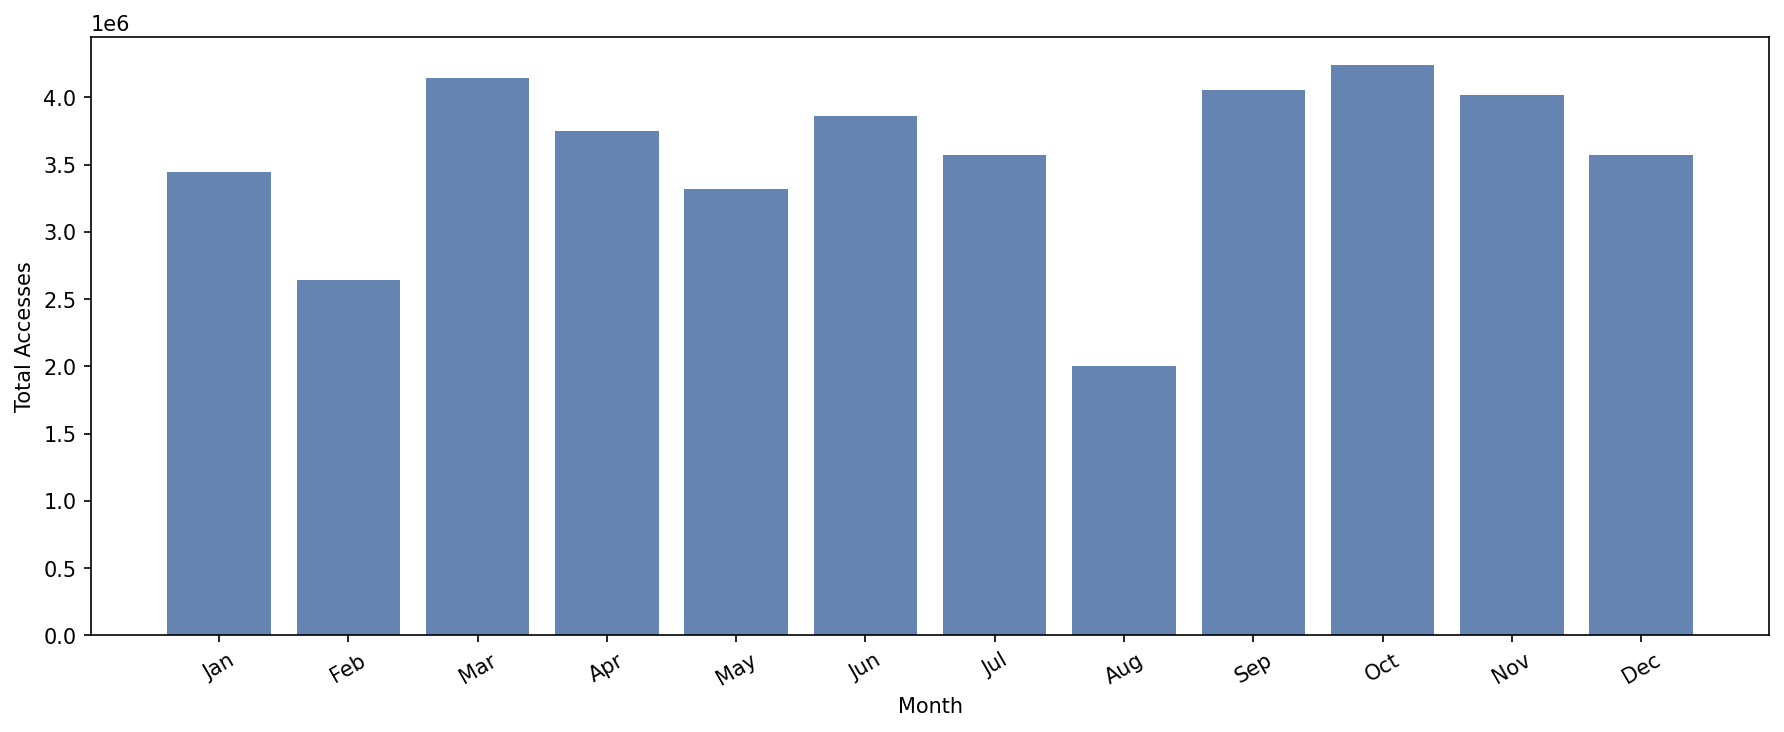
\includegraphics[width=0.7\textwidth]{./images/3_traffic/total_accesses_monthly.png}
	\end{figure}
	\begin{figure}[H]
		\centering
		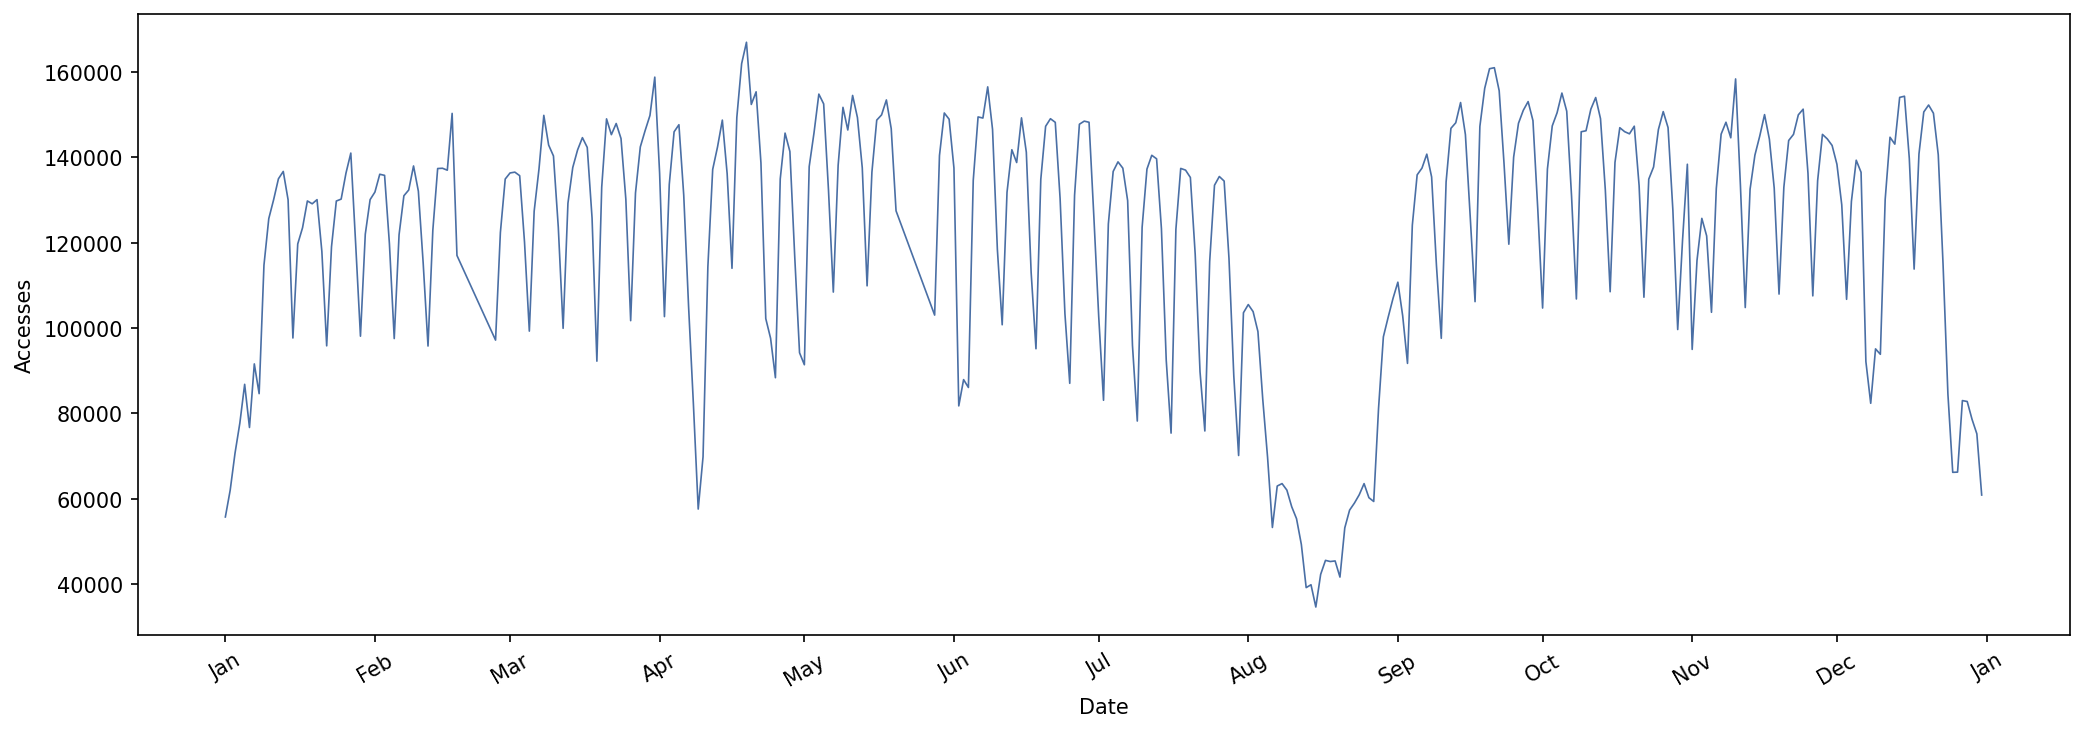
\includegraphics[width=0.7\textwidth]{./images/3_traffic/total_accesses_daily.png}
	\end{figure}
	
	Accesses peak in \textbf{October} and bottom out in \textbf{August}. 
	The daily series makes it clear that day-to-day swings come from a rigid \textbf{weekly cycle}, not from any gradual seasonal drift.
	
	\newpage
	\textbf{Fleet composition by fuel type} \\
	\begin{figure}[H]
		\centering
		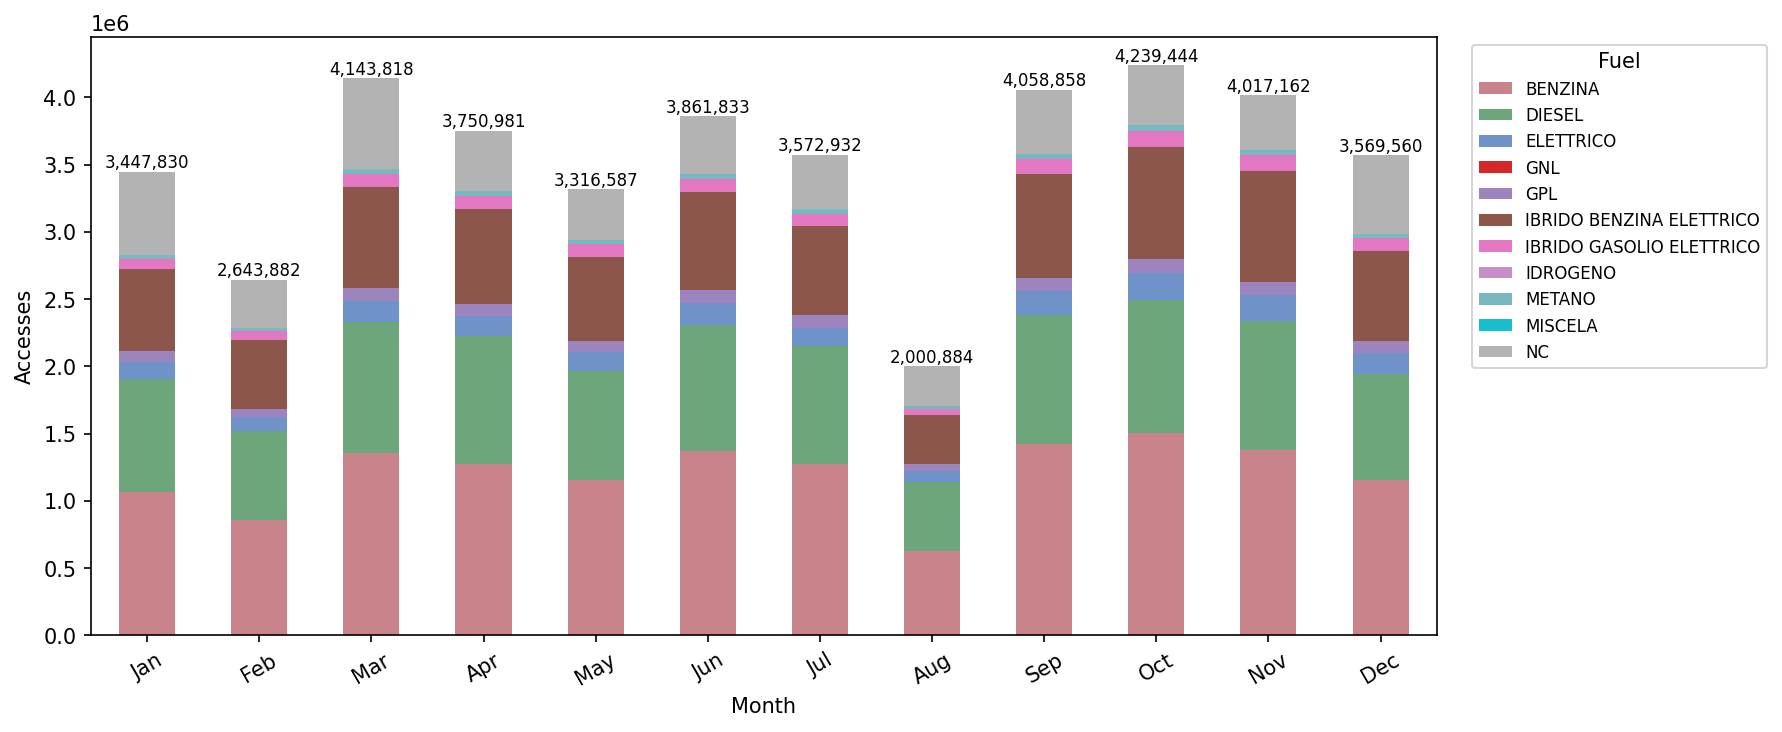
\includegraphics[width=0.7\textwidth]{./images/3_traffic/fleet_composition_by_fuel_monthly.png}
		\caption{Monthly fleet composition by fuel type.}
	\end{figure}
	
	\begin{figure}[H]
		\centering
		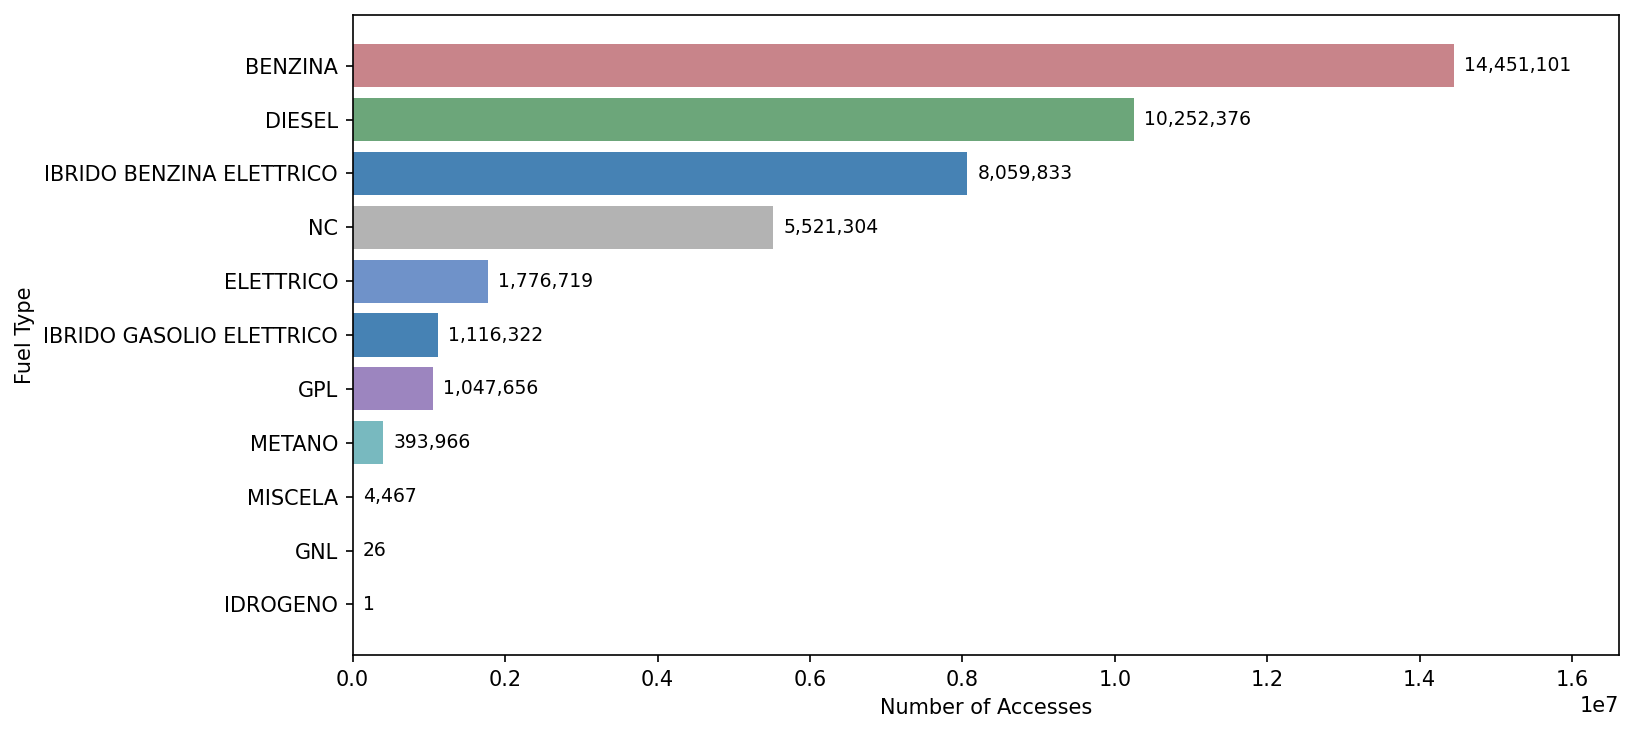
\includegraphics[width=0.7\textwidth]{./images/3_traffic/total_accesses_by_fuel.png}
		\caption{Total accesses by fuel type.}
	\end{figure}
	
	Benzina and Diesel together make up about 58\% of accesses, but \textbf{Ibrido Benzina Elettrico} already accounts for 19\%, pushing total low-emission share to roughly 23\%. 
	Alternative fuels are marginal ($<$3.5\%). Hydrogen: one single access all year. 
	The \textbf{NC} category (13\%) is large enough to be a real problem for any emission estimate built on fleet composition. 
	Month-to-month, the mix barely changes.

	\newpage
	\textbf{Fleet composition by Euro standard} \\
	\begin{figure}[H]
		\centering
		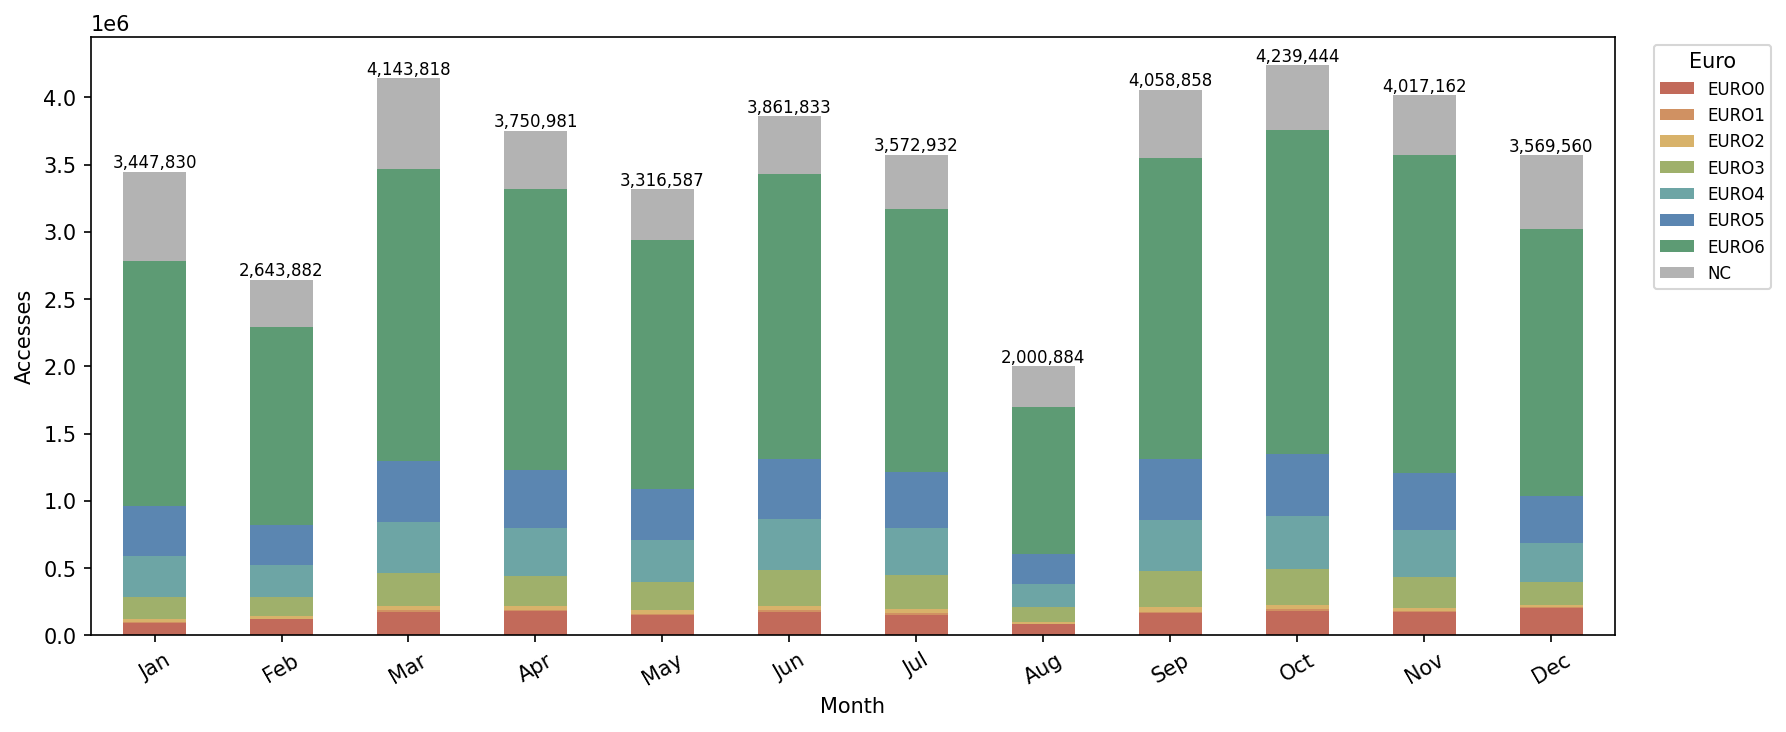
\includegraphics[width=0.8\textwidth]{./images/3_traffic/fleet_composition_by_euro_monthly.png}
		\caption{Monthly fleet composition by Euro standard.}
	\end{figure}
	
	\begin{figure}[H]
		\centering
		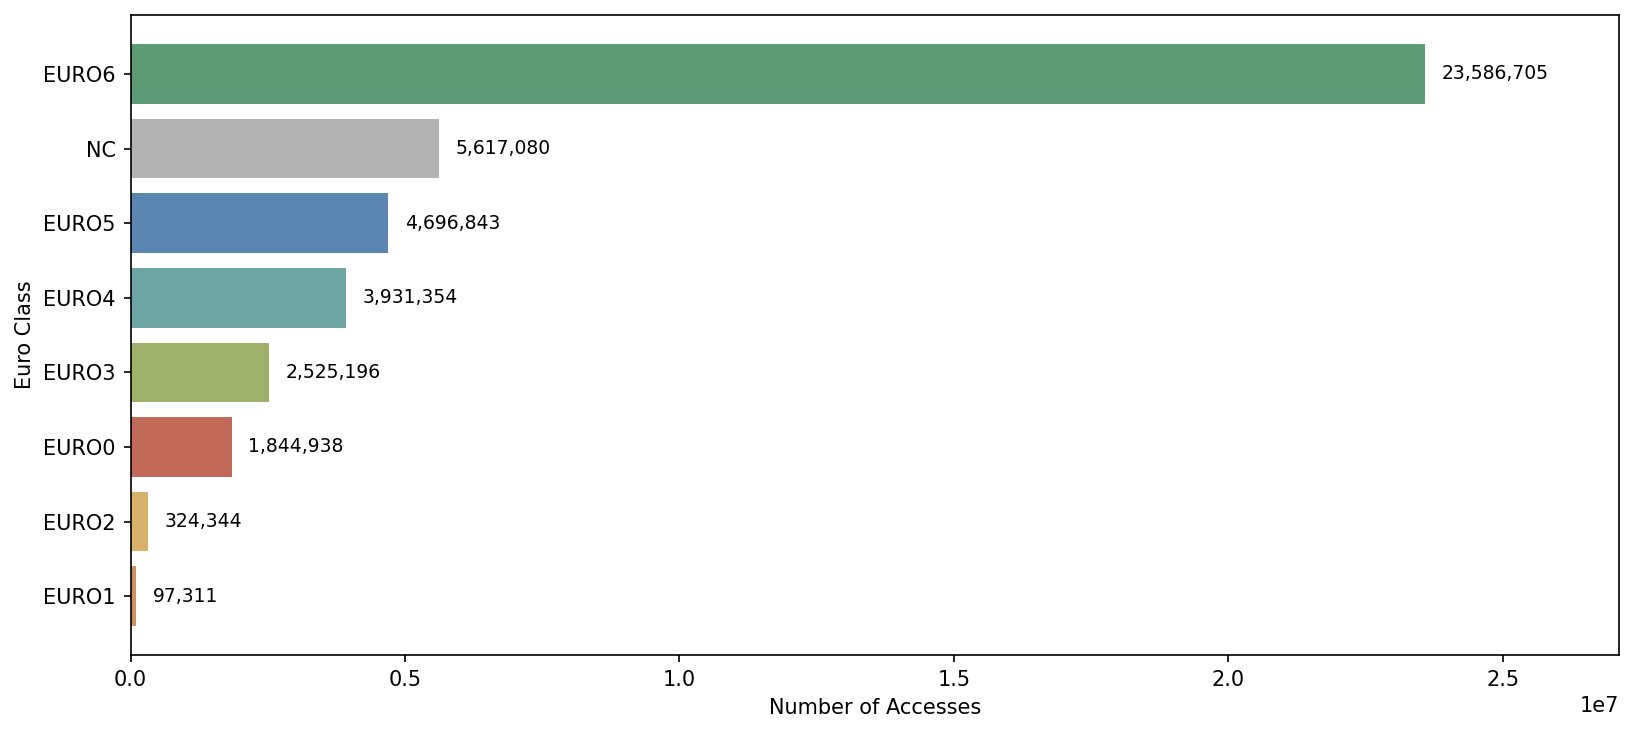
\includegraphics[width=0.8\textwidth]{./images/3_traffic/total_accesses_by_euro.png}
		\caption{Total accesses by Euro standard.}
	\end{figure}
	
	\textbf{Euro 6} vehicles make up over 55\% of accesses, a direct consequence of progressive urban access bans pushing fleet renewal.
	The \textbf{Euro 0} share (about 4\%) is actually higher than Euro 1 and Euro 2 combined, most likely motorcycles and historic vehicles benefiting from exemptions, not genuine non-compliance.

	\newpage
	\subsubsection{Can daily vehicle accesses be predicted?}
	
	A \textbf{Random Forest Regressor} was trained to predict daily accesses. 
	Features include lagged traffic (1, 2, 3, and 7 days back), a 7-day rolling mean and standard deviation, day of week, month, a weekend flag, a holiday and a bridge-day indicator.
	Hyperparameters were tuned by \textbf{Cross Validation} over an 11-fold \textbf{Time Series Split}, so every test fold comes strictly after its training data.
	
	\begin{figure}[H]
		\centering
		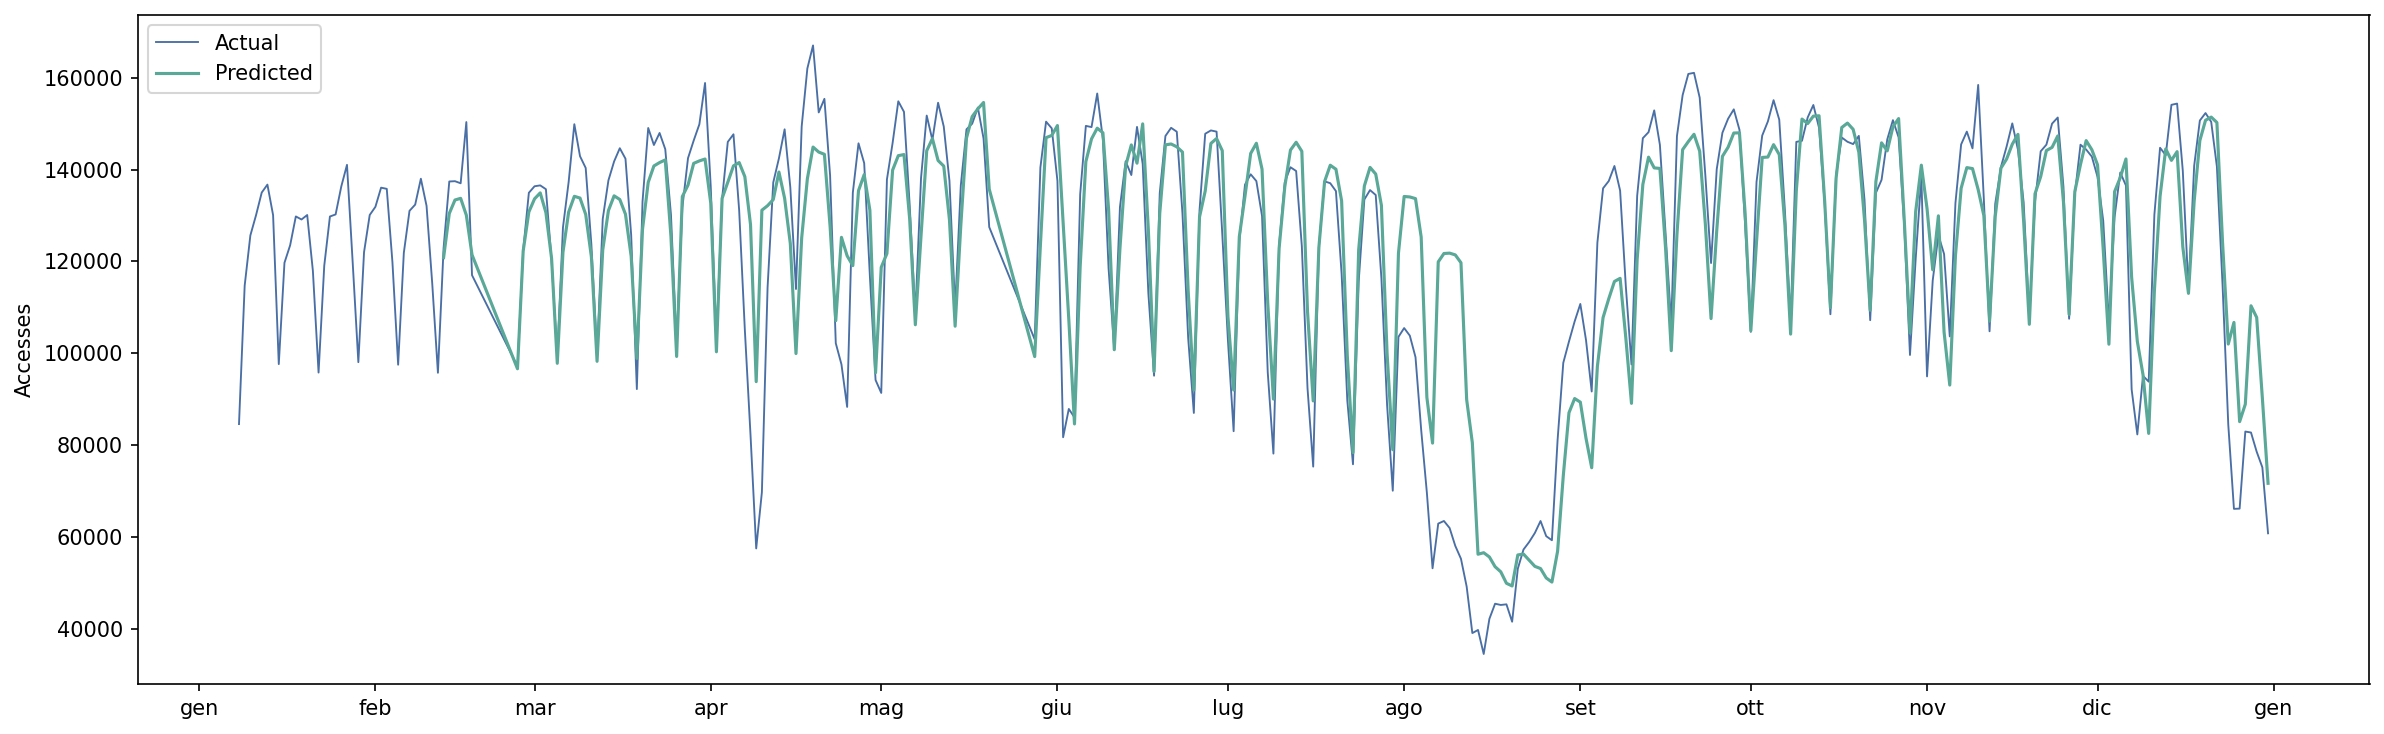
\includegraphics[width=0.9\textwidth]{./images/3_traffic/traffic_actual_vs_predicted.png}
			\caption{Actual vs. predicted daily traffic volumes.}
	\end{figure}
	\begin{figure}[H]
		\centering
		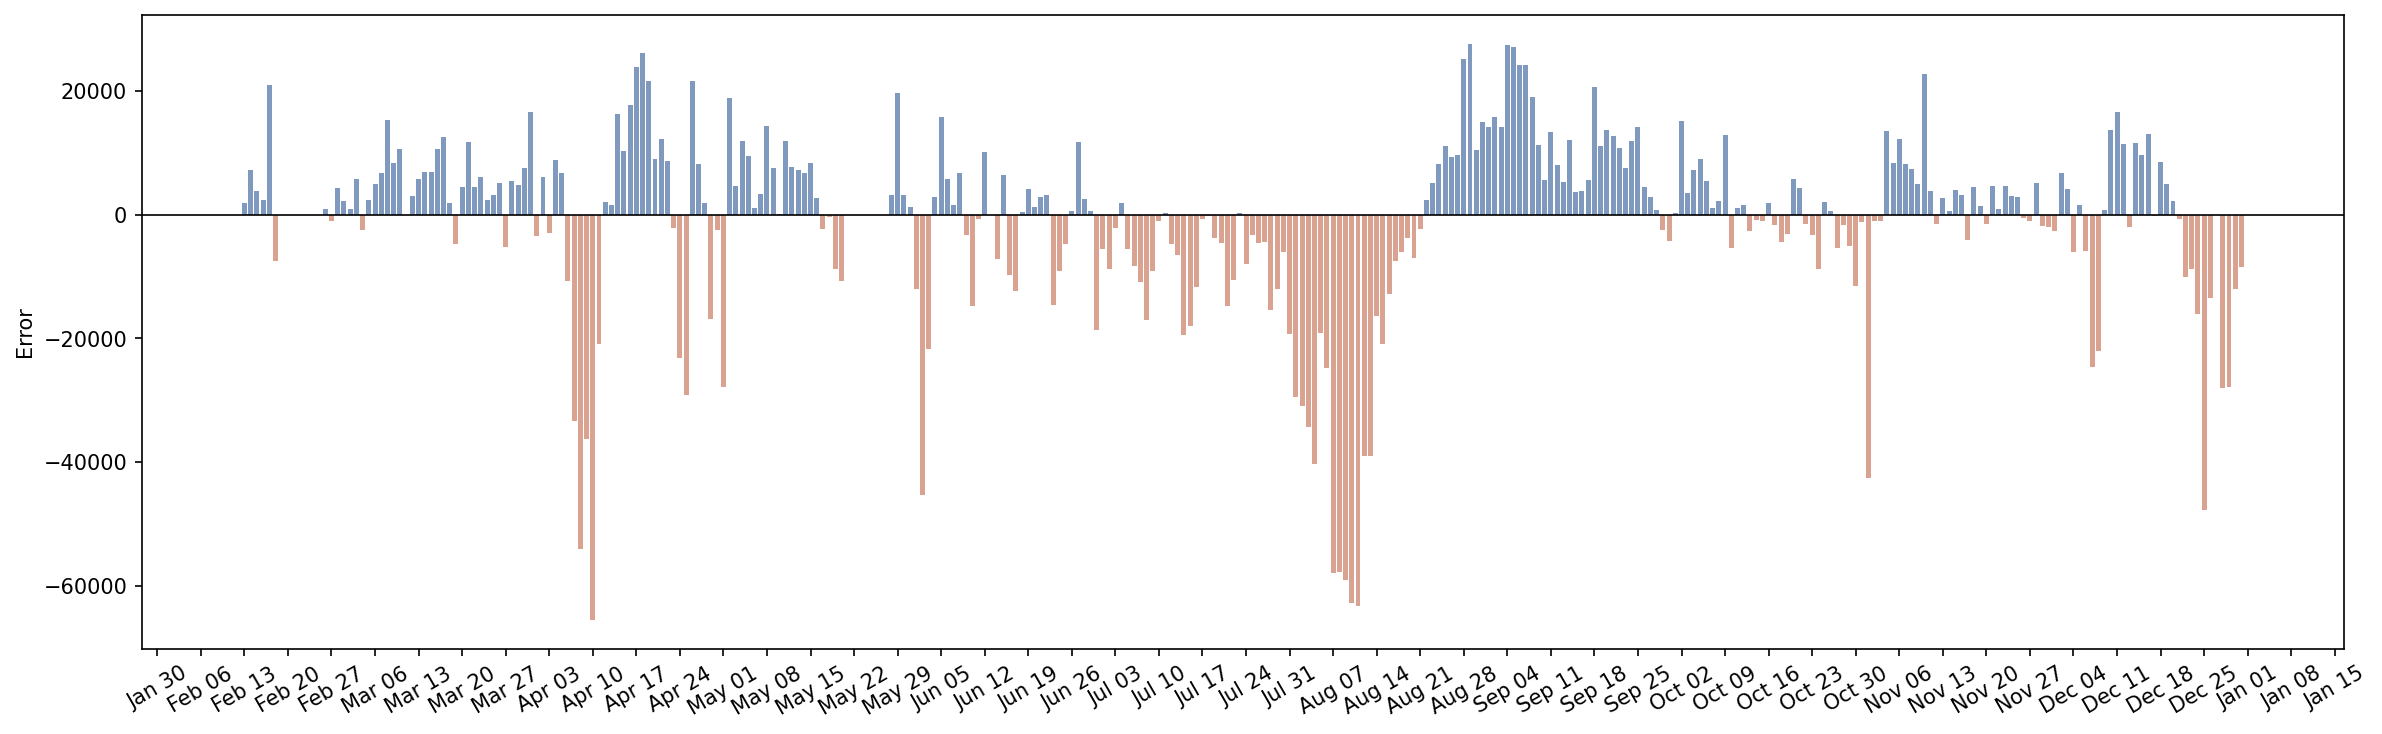
\includegraphics[width=0.9\textwidth]{./images/3_traffic/traffic_residuals.png}
		\caption{Residuals of the daily traffic volume predictions.}
	\end{figure}
	
	\begin{table}[H]
		\centering
		\begin{tabular}{ll}
			\hline
			Metric & Value \\
			\hline
			MAE & 10,666 accesses/day \\
			RMSE & 15,716 accesses/day \\
			MAPE & 11.2\% \\
			R$^2$ & 0.724 \\
			\hline
		\end{tabular}
	\end{table}
	
	The features capture about 72\% of daily variance. The missing 28\% is presumably related to other feature not mapped like weather, big public events, and transport strikes.
	The model over-predicts because its lag features carry forward normal working-day volumes and cannot anticipate the sudden drop. 
	Holiday and bridge-day indicators were added to compensate but is not sufficient.
	The mirror problem shows up on post-holiday return days where traffic rebounds sharply, producing the largest under-predictions. 

	\newpage
	\subsubsection{Which days show anomalous traffic volumes?}
	
	An \textbf{Isolation Forest} (200 estimators) was fitted on daily traffic totals.

	\begin{figure}[H]
		\centering
		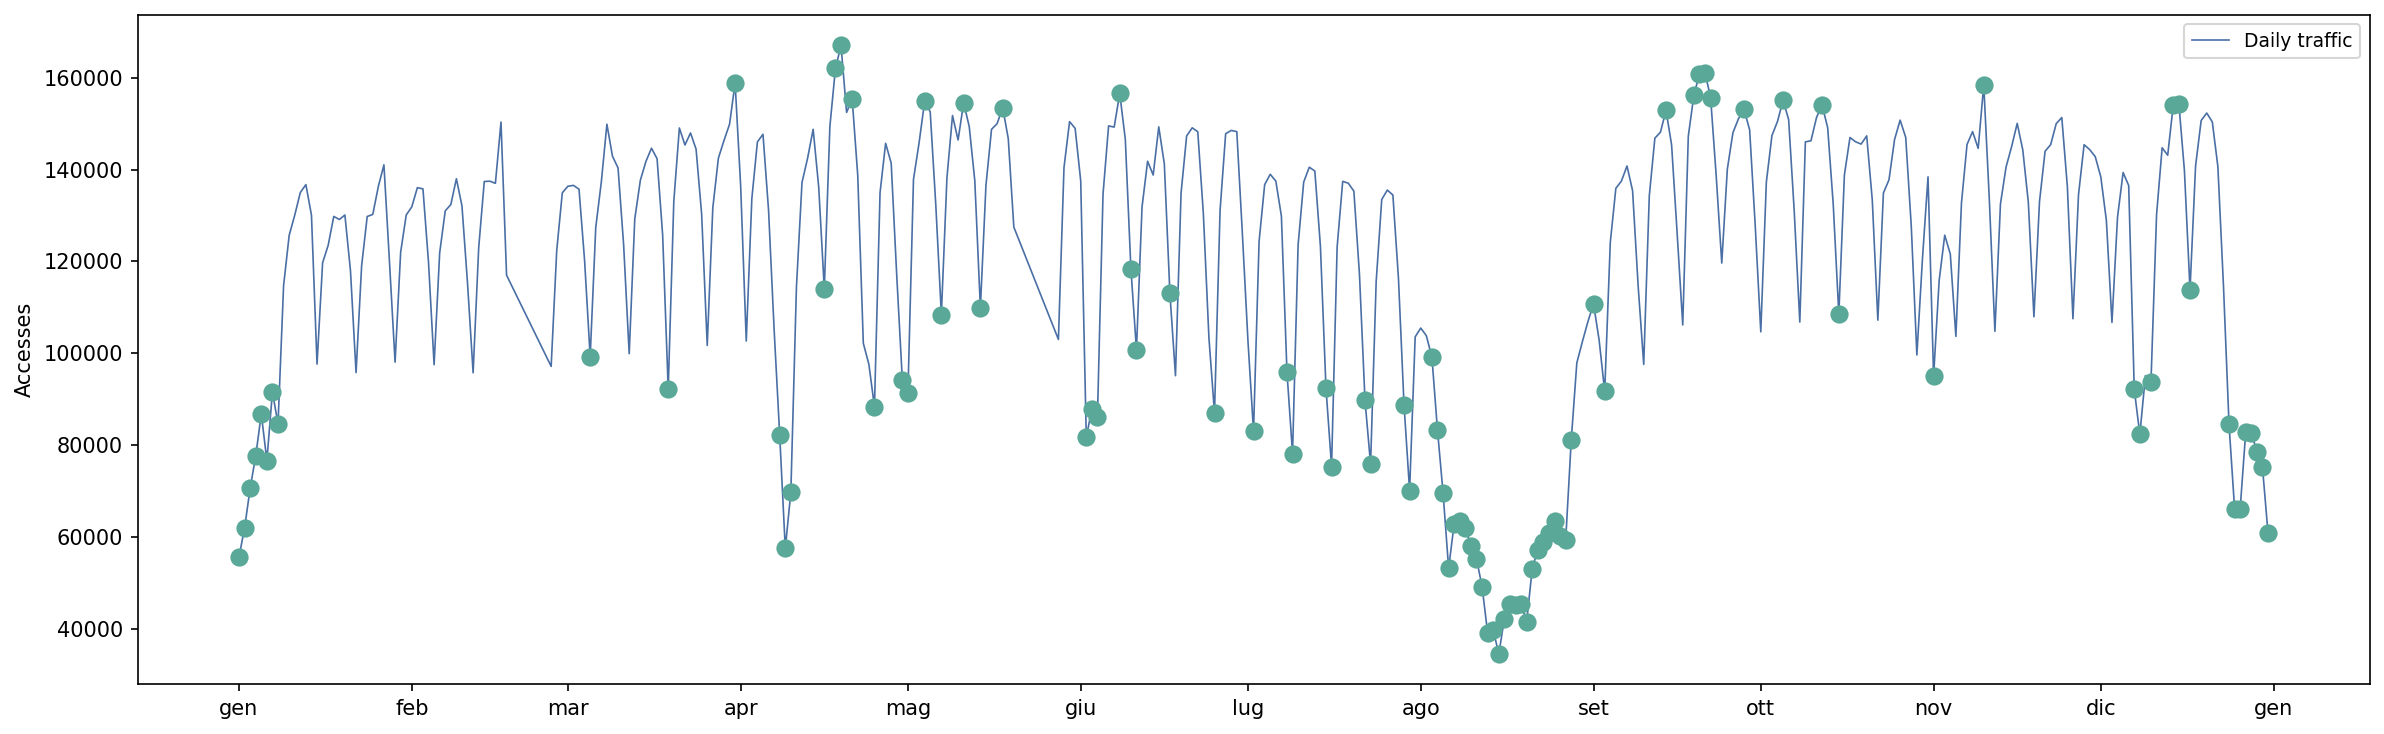
\includegraphics[width=0.9\textwidth]{./images/3_traffic/anomaly_isolation_forest.png}
		\caption{Isolation Forest anomaly detection results.}
	\end{figure}
	\begin{figure}[H]
		\centering
		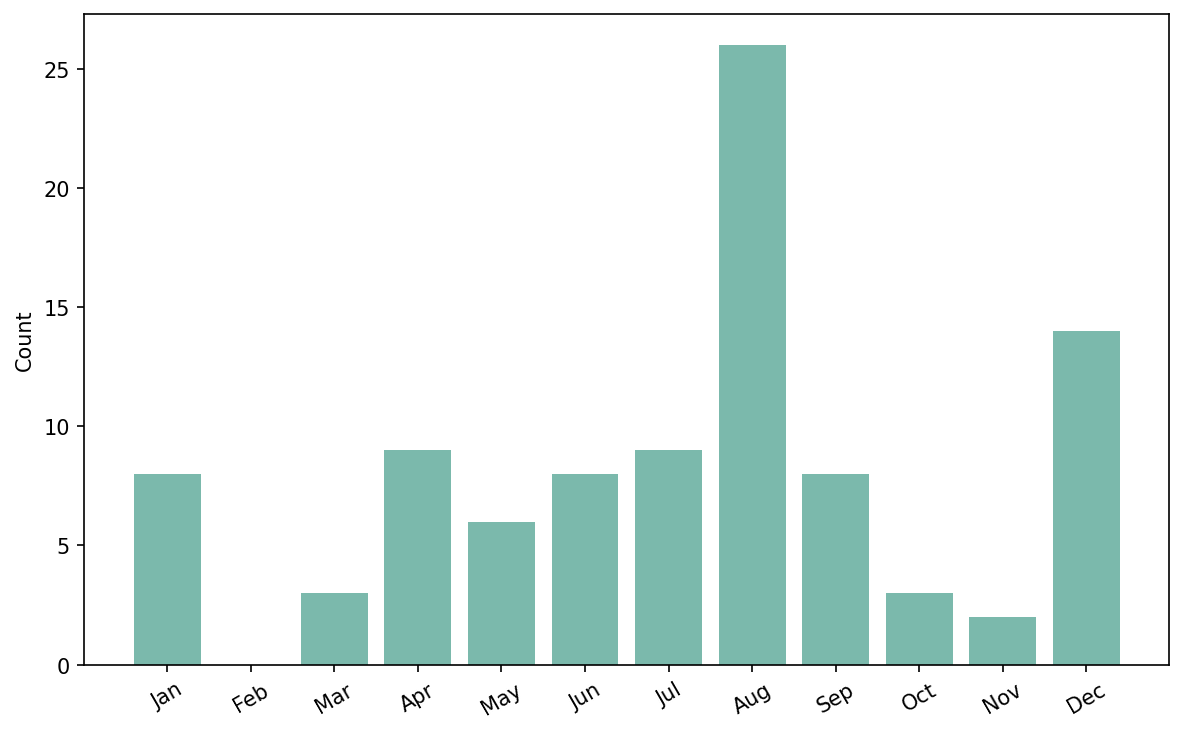
\includegraphics[width=0.4\textwidth]{./images/3_traffic/anomaly_by_month.png}s
		\caption{Monthly distribution of detected anomalies.}
	\end{figure}
	
	\textbf{96 days} were flagged, splitting neatly into three groups.
	The \textbf{extreme low-traffic anomalies} form the most visible cluster: the Ferragosto period in August, where daily volumes collapse.
	The \textbf{high-traffic anomalies} correspond to predictable demand peaks: the days around Easter in April, the end-of-summer rebound in September--October, and isolated Fridays before long weekends, where volumes spikess.
	The \textbf{low-traffic outliers} are scattered public holidays throughout the year, most visibly in January and December, where daily volumes goo down without reaching the extreme lows of August.
	Every flagged day has an obvious calendar explanation. Area C traffic is, in short, very regular once you account for a handful of known events.

	\newpage
	
	\subsection{Is there a measurable association between human activity intensity and air pollutant levels?}
	
	\subsubsection{Do high traffic days co-occur with elevated pollutant levels?}

	The activity variable here is \textbf{Area C daily traffic volume}, paired with daily concentrations of NO$_2$, O$_3$, PM$_{10}$, and PM$_{2.5}$.
	Because the traffic data covers only one zone, \textbf{this analysis is limited to the municipality of Milan}.
	Both traffic and pollutant values were binned into three levels (LOW, MID, HIGH) using tertiles over the Milan daily series.
	Apriori was run with minimum support 0.5\% and minimum confidence 20\%. 
	Only rules with a traffic-only antecedent, pollutant-only consequent, and lift $\geq$ 1.0 were kept.

	\begin{table}[H]
		\centering
		\resizebox{\textwidth}{!}{%
		\begin{tabular}{llrrr}
			\hline
			Antecedent & Consequent & Support & Confidence & Lift \\
			\hline
			\texttt{TRAFFIC\_LOW}& \texttt{NO2\_LOW + O3\_HIGH + PM10\_LOW}& 8.26\% & 24.8\% & 1.89 \\
			\texttt{TRAFFIC\_LOW}& \texttt{NO2\_LOW + O3\_HIGH}& 15.67\% & 47.0\% & 1.83 \\
			\texttt{TRAFFIC\_LOW}& \texttt{NO2\_LOW + O3\_HIGH + PM25\_MID}& 7.98\% & 23.9\% & 1.83 \\
			\texttt{TRAFFIC\_LOW}& \texttt{NO2\_LOW + PM25\_MID} & 8.83\% & 26.5\% & 1.82 \\
			\texttt{TRAFFIC\_LOW}& \texttt{NO2\_LOW + O3\_HIGH + PM25\_LOW}& 7.41\% & 22.2\% & 1.81 \\
			\texttt{TRAFFIC\_LOW}& \texttt{O3\_HIGH + PM10\_LOW + PM25\_LOW} & 6.84\% & 20.5\% & 1.80 \\
			\texttt{TRAFFIC\_LOW}& \texttt{O3\_HIGH + PM10\_LOW} & 8.55\% & 25.6\% & 1.80 \\
			\texttt{TRAFFIC\_LOW}& \texttt{NO2\_LOW + PM10\_LOW} & 11.40\% & 34.2\% & 1.79 \\
			\texttt{TRAFFIC\_LOW}& \texttt{NO2\_LOW + PM10\_LOW + PM25\_LOW} & 9.40\% & 28.2\% & 1.77 \\
			\texttt{TRAFFIC\_LOW}& \texttt{NO2\_LOW} & 19.37\% & 58.1\% & 1.74 \\
			\texttt{TRAFFIC\_LOW}& \texttt{O3\_HIGH + PM25\_LOW} & 7.69\% & 23.1\% & 1.72 \\
			\texttt{TRAFFIC\_HIGH} & \texttt{NO2\_MID + PM25\_MID} & 6.84\% & 20.5\% & 1.71 \\
			\texttt{TRAFFIC\_LOW}& \texttt{NO2\_LOW + PM10\_MID} & 6.84\% & 20.5\% & 1.71 \\
			\texttt{TRAFFIC\_LOW}& \texttt{NO2\_LOW + PM25\_LOW} & 10.26\% & 30.8\% & 1.66 \\
			\texttt{TRAFFIC\_LOW}& \texttt{O3\_HIGH} & 17.09\% & 51.3\% & 1.54 \\
			\texttt{TRAFFIC\_LOW}& \texttt{O3\_HIGH + PM25\_MID} & 8.26\% & 24.8\% & 1.47 \\
			\texttt{TRAFFIC\_MID}& \texttt{NO2\_HIGH + O3\_LOW + PM25\_HIGH} & 8.83\% & 26.5\% & 1.45 \\
			\texttt{TRAFFIC\_MID}& \texttt{NO2\_HIGH + O3\_LOW}& 11.11\% & 33.3\% & 1.44 \\
			\texttt{TRAFFIC\_MID}& \texttt{NO2\_HIGH + O3\_LOW + PM10\_HIGH} & 8.26\% & 24.8\% & 1.43 \\
			\texttt{TRAFFIC\_MID}& \texttt{NO2\_HIGH + O3\_LOW + PM10\_HIGH + PM25\_HIGH} & 7.98\% & 23.9\% & 1.42 \\
			\hline
		\end{tabular}}
		\caption*{Top 20 rules ranked by lift (Traffic $\rightarrow$ Pollutants).}
	\end{table}

	Three traffic patterns emerge from the rules, but none reflects a direct causal link with emissions.

	The \texttt{TRAFFIC\_LOW} rules dominate the top of the table. The strongest, \texttt{TRAFFIC\_LOW $\rightarrow$ NO2\_LOW + O3\_HIGH + PM10\_LOW} (lift 1.89), and the rest of the \texttt{TRAFFIC\_LOW} group (lifts 1.54--1.83) all point to the same \texttt{NO2\_LOW + O3\_HIGH} signature. 
	This can be \textbf{seasonal confounding}, low traffic and high ozone co-occur because mainly because August kills commuter traffic exactly when summer meteorology pushes O$_3$ up.
	
	The \texttt{TRAFFIC\_MID} pattern captures the opposite season. 
	Rule \texttt{TRAFFIC\_MID $\rightarrow$ NO2\_HIGH + O3\_LOW + PM25\_HIGH} (lift 1.45) anchors a tight group (lifts 1.42--1.45) where intermediate volumes pair with elevated NO$_2$ and PM$_{2.5}$. 
	This matches autumn and winter workdays, when \textbf{atmospheric stagnation} traps pollutants.

	The \texttt{TRAFFIC\_HIGH} pattern yields a single rule, \texttt{TRAFFIC\_HIGH $\rightarrow$ NO2\_MID + PM25\_MID} (lift 1.71): peak volumes produce no distinctive pollution signature beyond what the season already explains.

	The overall maximum lift of 1.89 is low by association-rule standards. Two structural limitations apply. 

	First, \textbf{geography}: traffic and pollution data are both restricted to Milan, so nothing here generalizes to the rest of Lombardia. 

	Second, \textbf{instrument mismatch}: Area C monitors a single corridor into the city centre and captures only a fraction of total urban mobility, making it a weak proxy for actual emission intensity. 

	A more effective analysis would need region-wide counts from motorways, provincial roads, and other cities.

	\newpage
	\subsubsection{Does high tourism pressure co-occur with higher pollution levels?}

	Here the activity variable is the \textbf{monthly tourism pressure index}, compared against daily concentrations of NO$_2$, O$_3$, PM$_{10}$, and PM$_{2.5}$.
	Tourism data is natively monthly, so both activity and pollution were discretized into LOW, MID, HIGH using \textbf{per-municipality monthly tertiles}. 
	Apriori ran with minimum support 0.5\% and minimum confidence 20\%, keeping only rules with lift $\geq$ 1.0, tourism-only antecedent, and pollutant-only consequent.

	\begin{table}[H]
		\centering
		\resizebox{\textwidth}{!}{%
		\begin{tabular}{llrrr}
			\hline
			Antecedent & Consequent & Support & Confidence & Lift \\
			\hline
			\texttt{TOURISM\_LOW}& \texttt{O3\_LOW + PM10\_HIGH + PM25\_HIGH} & 6.87\% & 20.5\% & 2.65 \\
			\texttt{TOURISM\_LOW}& \texttt{NO2\_HIGH + PM10\_HIGH + PM25\_HIGH} & 8.93\% & 26.7\% & 2.63 \\
			\texttt{TOURISM\_LOW}& \texttt{PM10\_HIGH + PM25\_HIGH}& 9.97\% & 29.7\% & 2.55 \\
			\texttt{TOURISM\_LOW}& \texttt{O3\_LOW + PM25\_HIGH} & 7.22\% & 21.5\% & 2.51 \\
			\texttt{TOURISM\_LOW}& \texttt{NO2\_HIGH + O3\_LOW + PM25\_HIGH} & 6.87\% & 20.5\% & 2.49 \\
			\texttt{TOURISM\_LOW}& \texttt{NO2\_HIGH + O3\_LOW + PM10\_HIGH} & 10.48\% & 31.3\% & 2.40 \\
			\texttt{TOURISM\_LOW}& \texttt{O3\_LOW + PM10\_HIGH} & 11.17\% & 33.3\% & 2.40 \\
			\texttt{TOURISM\_LOW}& \texttt{NO2\_HIGH + PM25\_HIGH} & 9.62\% & 28.7\% & 2.39 \\
			\texttt{TOURISM\_LOW}& \texttt{NO2\_HIGH + PM10\_HIGH} & 15.81\% & 47.2\% & 2.33 \\
			\texttt{TOURISM\_LOW}& \texttt{PM25\_HIGH} & 10.82\% & 32.3\% & 2.29 \\
			\texttt{TOURISM\_LOW}& \texttt{NO2\_HIGH + O3\_LOW}& 14.09\% & 42.1\% & 2.13 \\
			\texttt{TOURISM\_LOW}& \texttt{PM10\_HIGH} & 17.87\% & 53.3\% & 2.07 \\
			\texttt{TOURISM\_LOW}& \texttt{O3\_LOW}& 15.64\% & 46.7\% & 2.01 \\
			\texttt{TOURISM\_LOW}& \texttt{NO2\_HIGH}& 22.34\% & 66.7\% & 2.00 \\
			\texttt{TOURISM\_HIGH} & \texttt{NO2\_LOW + O3\_HIGH}& 11.51\% & 34.5\% & 1.72 \\
			\texttt{TOURISM\_HIGH} & \texttt{O3\_HIGH} & 12.37\% & 37.1\% & 1.64 \\
			\texttt{TOURISM\_HIGH} & \texttt{NO2\_LOW} & 18.21\% & 54.6\% & 1.63 \\
			\texttt{TOURISM\_HIGH} & \texttt{NO2\_LOW + PM10\_LOW} & 10.14\% & 30.4\% & 1.58 \\
			\texttt{TOURISM\_HIGH} & \texttt{PM25\_MID}& 7.22\% & 21.6\% & 1.56 \\
			\texttt{TOURISM\_HIGH} & \texttt{NO2\_MID + PM10\_MID} & 6.87\% & 20.6\% & 1.48 \\
			\hline
		\end{tabular}}
		\caption*{Top 20 rules ranked by lift (Tourism $\rightarrow$ Pollutants).}
	\end{table}

	Two tourism patterns emerge from the rules, but both reduce to seasonal weather rather than visitor activity.

	The \texttt{TOURISM\_LOW} rules fill 14 of the top 20 slots. The strongest, \texttt{TOURISM\_LOW $\rightarrow$ O3\_LOW + PM10\_HIGH + PM25\_HIGH} (lift 2.65), anchors a tight group (lifts 2.00--2.65) that maps onto the classic winter fingerprint: \texttt{NO2\_HIGH}, \texttt{PM10\_HIGH}, \texttt{PM25\_HIGH}, \texttt{O3\_LOW}. The single highest-confidence rule, \texttt{TOURISM\_LOW $\rightarrow$ NO2\_HIGH} (66.7\%), confirms the picture. This is \textbf{thermal inversion} in winter, not an effect of fewer tourists.

	The \texttt{TOURISM\_HIGH} pattern captures the opposite season. Rule \texttt{TOURISM\_HIGH $\rightarrow$ NO2\_LOW + O3\_HIGH} (lift 1.72) anchors a smaller group (6 rules, lifts 1.48--1.72) pairing peak visitor months with the photochemical signature of summer: low NO$_2$ and high O$_3$, exactly what high radiation and better ventilation produce. No rules link high tourism to pollution levels above what the season already generates.

	Two structural limitations weaken these patterns. 
	
	First, \textbf{temporal granularity}: tourism is reported monthly, so every day within a month inherits the same \texttt{TOURISM\_LOW}/\texttt{MID}/\texttt{HIGH} label. 
	Daily variability in the antecedent is gone, and the rules effectively reduce to a comparison between calendar months. 
	The high lifts (up to 2.65) reflect the strong seasonal contrast in pollution, not a sharp dependence on visitor numbers. 
	
	Second, the monthly index conflates \textbf{season and tourism intensity}: low-tourism months are also winter months, so the antecedent cannot be cleanly separated from the meteorology it correlates with.

	Tourism intensity therefore acts as a \textbf{calendar proxy}. 
	No rule connects high visitor numbers to pollution levels above what the season already produces, and municipality-scale air quality is driven by large-scale meteorology, not visitor counts. 
	A finer-grained tourism signal (daily arrivals, overnight stays) would be needed to test whether visitor pressure has any residual effect once seasonality is controlled for.
	\newpage
	
	\section{Generative artificial intelligence tools used}

	AI tools like GitHub Copilot and Google Gemini were used during the project for:
	\begin{itemize}
		\item support writing and debugging python code
		\item support writing documentation, checking text and fixing grammar
	\end{itemize}

	
\end{document}